\chapter{Object detection}


\begin{description}
    \item[Object detection] \marginnote{Object detection}
        Given an RGB $W \times H$ image, determine a set of objects $\{ o_1, \dots, o_n \}$ contained in it. Each object $o_j$ is described by:
        \begin{itemize}
            \item A category $c_j \in \{ 1, \dots, C \}$ as in image classification.
            \item A bounding box $BB_j = [ x_j, y_j, w_j, h_j ]$ where $x_j, w_j \in [0, W-1]$ and $y_j, h_j \in [0, H-1]$. ($x_j$, $y_j$) is the center and ($w_j$, $h_j$) is the size of the box.
            \item A confidence score $\rho_j$.
        \end{itemize}

        \begin{figure}[H]
            \centering
            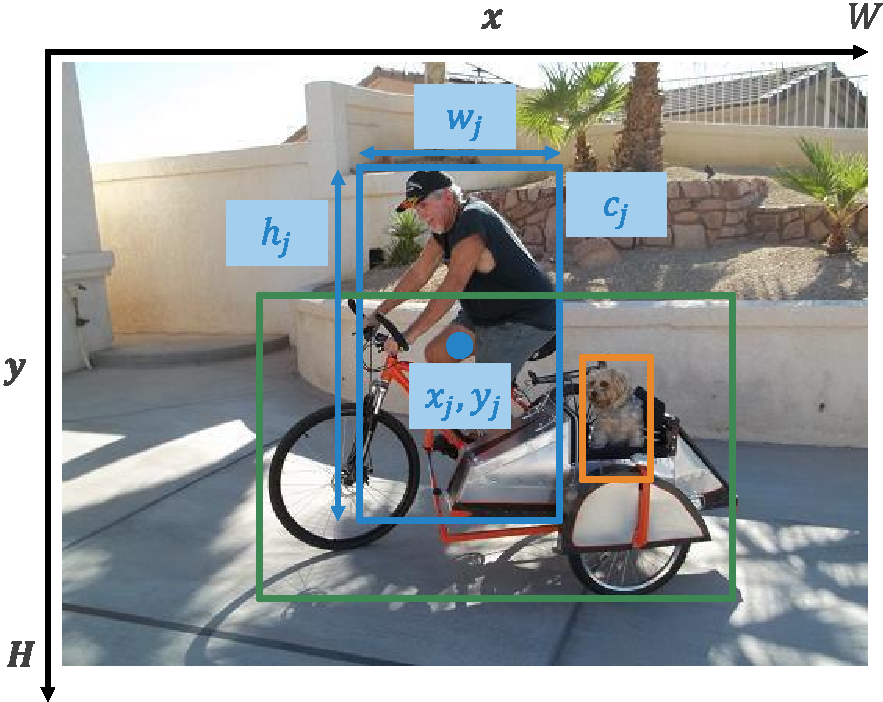
\includegraphics[width=0.45\linewidth]{./img/_object_detection_example.pdf}
        \end{figure}

        \begin{remark}
            Differently from classification, a model has to:
            \begin{itemize}
                \item Be able to output a variable number of results.
                \item Output both categorical and spatial information.
                \item Work on high resolution input images.
            \end{itemize}
        \end{remark}
\end{description}



\section{Metrics}

\begin{description}
    \item[Intersection over union (\texttt{IoU})] 
    \marginnote{Intersection over union (\texttt{IoU})}
        Measures the amount of overlap between two boxes computed as the ratio of the area of intersection over the area of union:
        \[ \texttt{IoU}(BB_i, BB_j) = \frac{\vert BB_i \cap BB_j \vert}{\vert BB_i \vert + \vert BB_j \vert - \vert BB_i \cup BB_j \vert} \]

        \begin{description}
            \item[True/false positive criteria] 
                Given a threshold $\rho_\texttt{IoU}$, a detection $BB_i$ is a true positive (\texttt{TP}) w.r.t. a ground-truth $\widehat{BB_j}$ if it is classified with the same class and:
                \[ \texttt{IoU}(BB_i, \widehat{BB_j}) > \rho_\texttt{IoU} \]

                \begin{remark}
                    Confidence can also be considered when determining a match through a threshold $\rho_\text{min}$.
                \end{remark}
        \end{description}

    \item[Recall]
        Measures the number of ground-truth objects that have been found:
        \[ \texttt{recall} = \frac{\vert \texttt{TP} \vert}{\vert \text{ground-truth boxes} \vert} \]

    \item[Precision]
        Measures the number of correct detections among all the predictions:
        \[ \texttt{precision} = \frac{\vert \texttt{TP} \vert}{\vert \text{model detections} \vert} \]

    \begin{figure}[H]
        \centering
        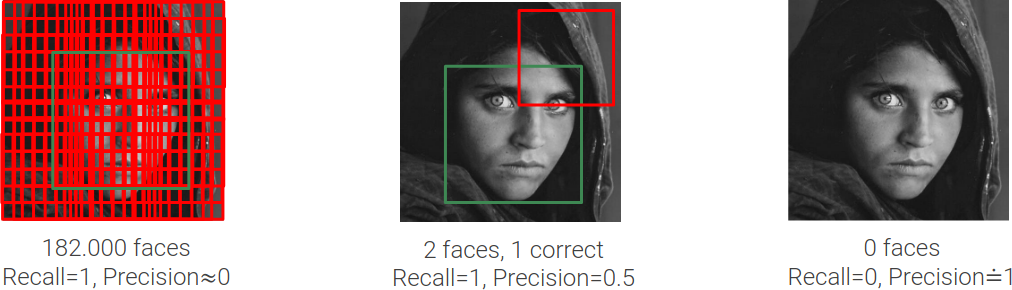
\includegraphics[width=0.7\linewidth]{./img/obj_det_recall_precision.png}
        \caption{
            Recall and precision in different scenarios
        }
    \end{figure}

    \item[Precision-recall curve]
        Plot that relates all possible precisions and recalls of a detector.

        \begin{example}
            Consider the following image and the bounding boxes found by a detector:
            \begin{figure}[H]
                \centering
                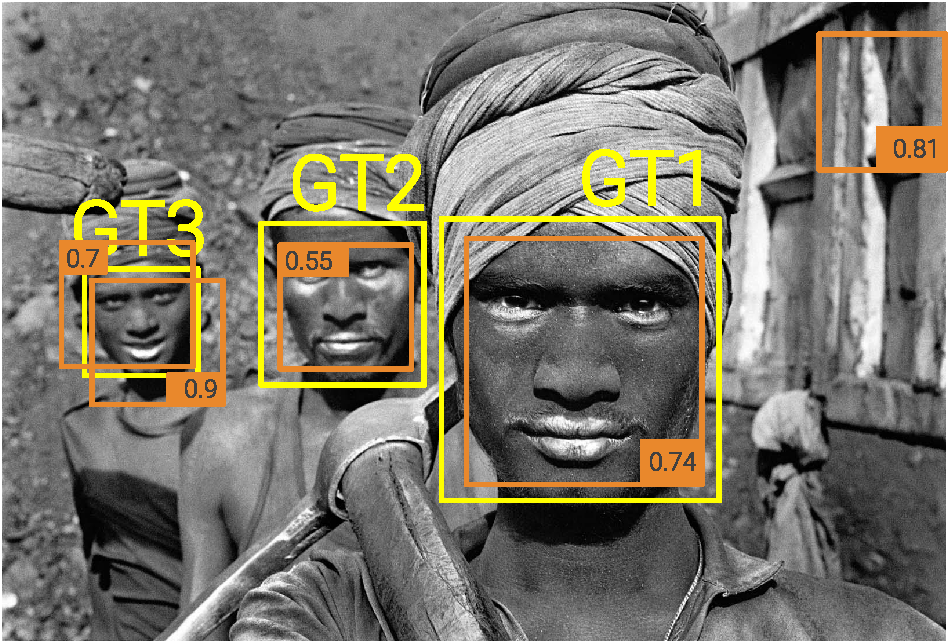
\includegraphics[width=0.4\linewidth]{./img/_example_precision_recall_curve1.pdf}
                \caption{
                    \parbox[t]{0.6\linewidth}{
                        Ground-truth (yellow boxes) and predictions (orange boxes) with their confidence score
                    }
                }
            \end{figure}

            By sorting the confidence scores, it is possible to plot the precision-recall curve by varying the threshold $\rho_\text{min}$:
            \begin{figure}[H]
                \centering
                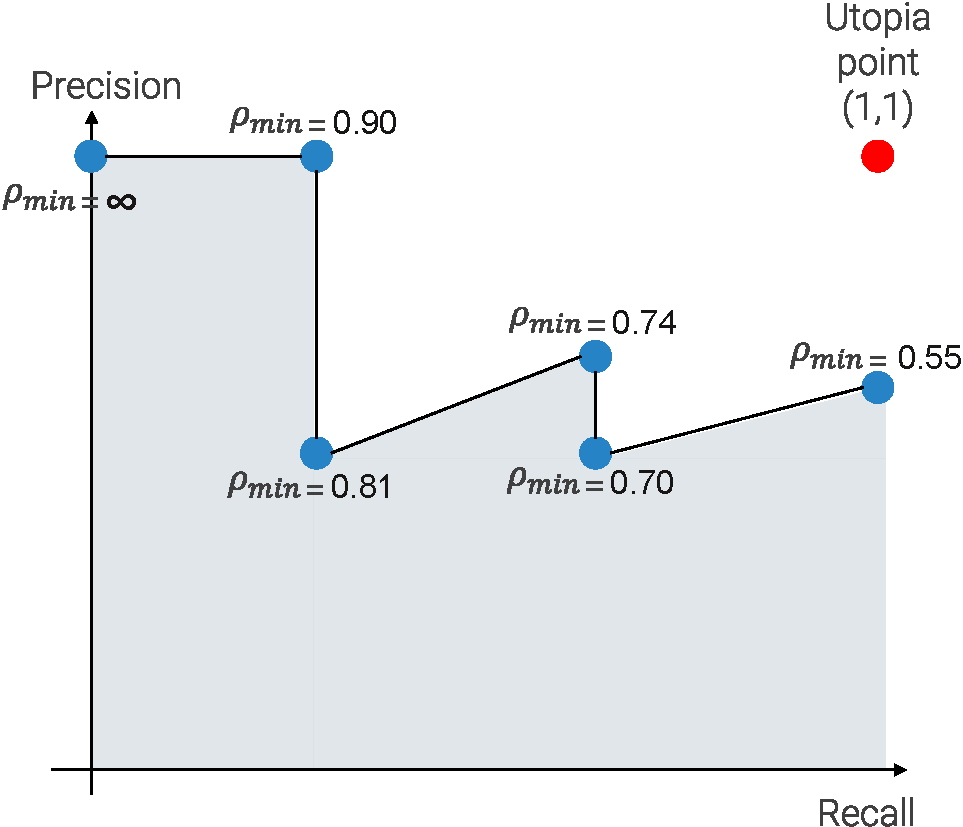
\includegraphics[width=0.4\linewidth]{./img/_example_precision_recall_curve2.pdf}
            \end{figure}

            \indenttbox
            \begin{remark}
                Recall is monotonically decreasing, while precision can both decrease and increase.
            \end{remark}
        \end{example}

        \begin{description}
            \item[Average precision (AP)] \marginnote{Average precision (AP)}
                Area under the precision-recall curve.

            \item[Mean average precision (mAP)] \marginnote{Mean AP (mAP)}
                Mean AP over the possible classes.

            \item[COCO mean average precision] \marginnote{COCO mAP}
                Compute for each class the average AP over varying $\rho_\texttt{IoU}$ (e.g., in the original paper, $\rho_\texttt{IoU} \in [0.5, 0.95]$ with $0.05$ steps) and further average them over the possible classes.

                \begin{remark}
                    Higher COCO mAP indicates a detector with good localization capabilities.
                \end{remark}
        \end{description}
\end{description}



\section{Viola-Jones}

\begin{description}
    \item[Viola-Jones] \marginnote{Viola-Jones object detection}
        General framework for object detection, mainly applied to faces.

        It is one of the first successful applications of machine learning in computer vision and has the following basis:
        \begin{itemize}
            \item Use AdaBoost to learn an ensemble of features.
            \item Use multi-scale rectangular features computed efficiently using integral images.
            \item Cascade to obtain real-time speed.
        \end{itemize}
\end{description}


\subsection{Boosting}

\begin{description}
    \item[Weak learner] \marginnote{Weak learner}
        Classifier with an error rate slightly higher than a random classifier (i.e., in a balanced binary task, accuracy slightly higher than $50\%$).

        \begin{description}
            \item[Decision stump] \marginnote{Decision stump}
                Classifier that learns a threshold for a single feature (i.e., decision tree with depth 1).
        \end{description}

    \item[Strong learner] \marginnote{Strong learner}
        Classifier with an accuracy strongly correlated with the ground-truth.

    \item[Adaptive boosting (AdaBoost)] \marginnote{Adaptive boosting (AdaBoost)}
        Ensemble of $M$ weak learners $\texttt{WL}_i$ that creates a strong learner $\texttt{SL}$ as the linear combination of their predictions (i.e., weighted majority vote):
        \[ \texttt{SL}(x) = \left( \sum_{i=1}^{M} \alpha_i \texttt{WL}_i(x) > 0 \right) \]

    \item[Training] \marginnote{Boosting training}
        Given $N$ training samples $(x^{(i)}, y^{(i)})$ and $M$ untrained weak learners $\texttt{WL}_i$, training is done sequentially by tuning a learner at the time:
        \begin{enumerate}
            \item Uniformly weigh each sample: $w^{(i)} = \frac{1}{N}$.
            \item For each weak learner $\texttt{WL}_j$ ($j=1, \dots, M$):
            \begin{enumerate}
                \item Fit the weak learner on the weighted training data.
                \item Compute its error rate:
                \[ \varepsilon_j = \sum_{i: x^{(i)} \text{ misclassified}} w^{(i)} \]
                \item Compute the reweigh factor:
                \[ \beta_j = \frac{1 - \varepsilon_j}{\varepsilon_j} \]
                \item Increase the weight of misclassified samples:
                \[ w^{(i)} = w^{(i)} \beta_j \]
                and re-normalize all samples so that their weights sum to $1$.
            \end{enumerate}
            \item Define the strong classifier as:
            \[ \texttt{SL}(x) = \left( \sum_{j} \ln(\beta_j) \texttt{WL}_j(x) > 0 \right) \]
        \end{enumerate}

        \begin{example}
            \small
            Consider the problem of spam detection with two features $x_1$ and $x_2$ (number of URL and capitalized words, respectively).
            The training samples and their initial weights are the following:
            \begin{figure}[H]
                \centering
                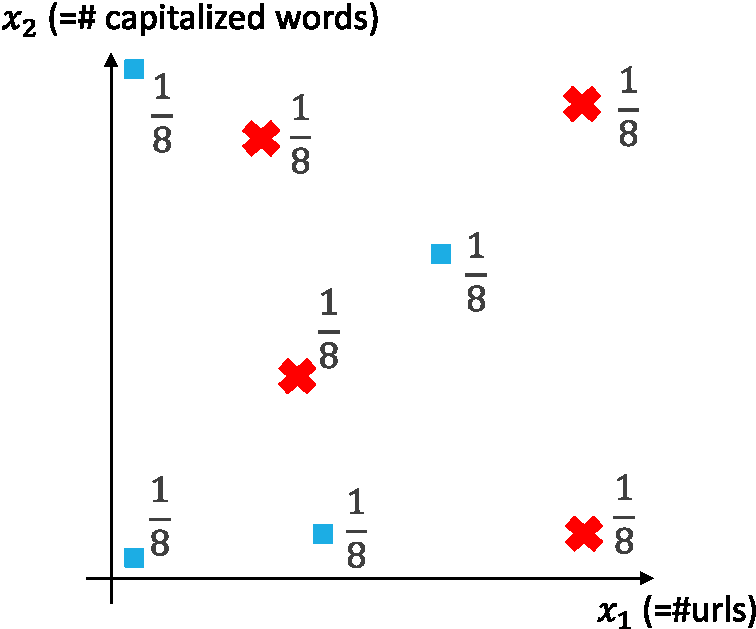
\includegraphics[width=0.3\linewidth]{./img/_adaboost_example1.pdf}
            \end{figure}
            We want to train an ensemble of $3$ decision stumps $\texttt{WL}_{j}$.

            Let's say that the first weak classifier learns to detect spam using the criteria $x_1 > 3$. The error rate and reweigh factor are:
            \[
                \varepsilon_1 = \frac{1}{8} + \frac{1}{8} \qquad
                \beta_1 = \frac{1 - \varepsilon_1}{\varepsilon_1} = 3
            \]
            The new reweighed and normalized samples are:
            \begin{figure}[H]
                \centering
                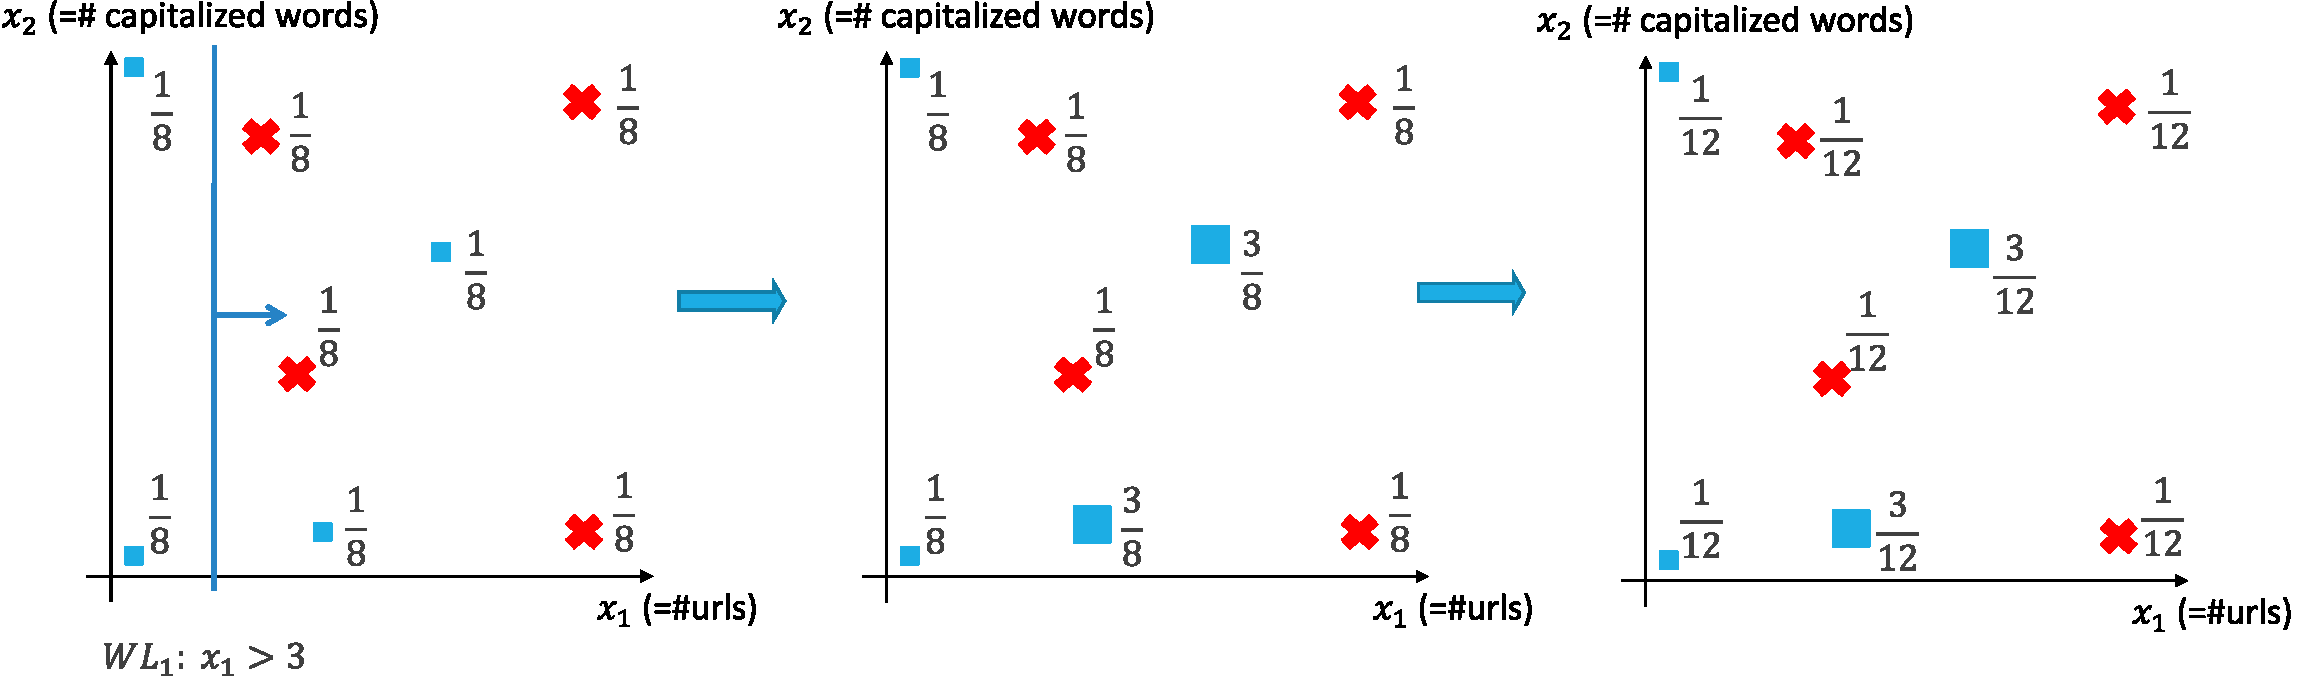
\includegraphics[width=0.9\linewidth]{./img/_adaboost_example2.pdf}
            \end{figure}

            Now, assume that the second classifier learns $x_1 > 10$. The error rate and reweigh factor are:
            \[ \varepsilon_2 = \frac{1}{12} + \frac{1}{12} \qquad
            \beta_2 = \frac{1 - \varepsilon_2}{\varepsilon_2} = 5 \]
            The new reweighed and normalized samples are:
            \begin{figure}[H]
                \centering
                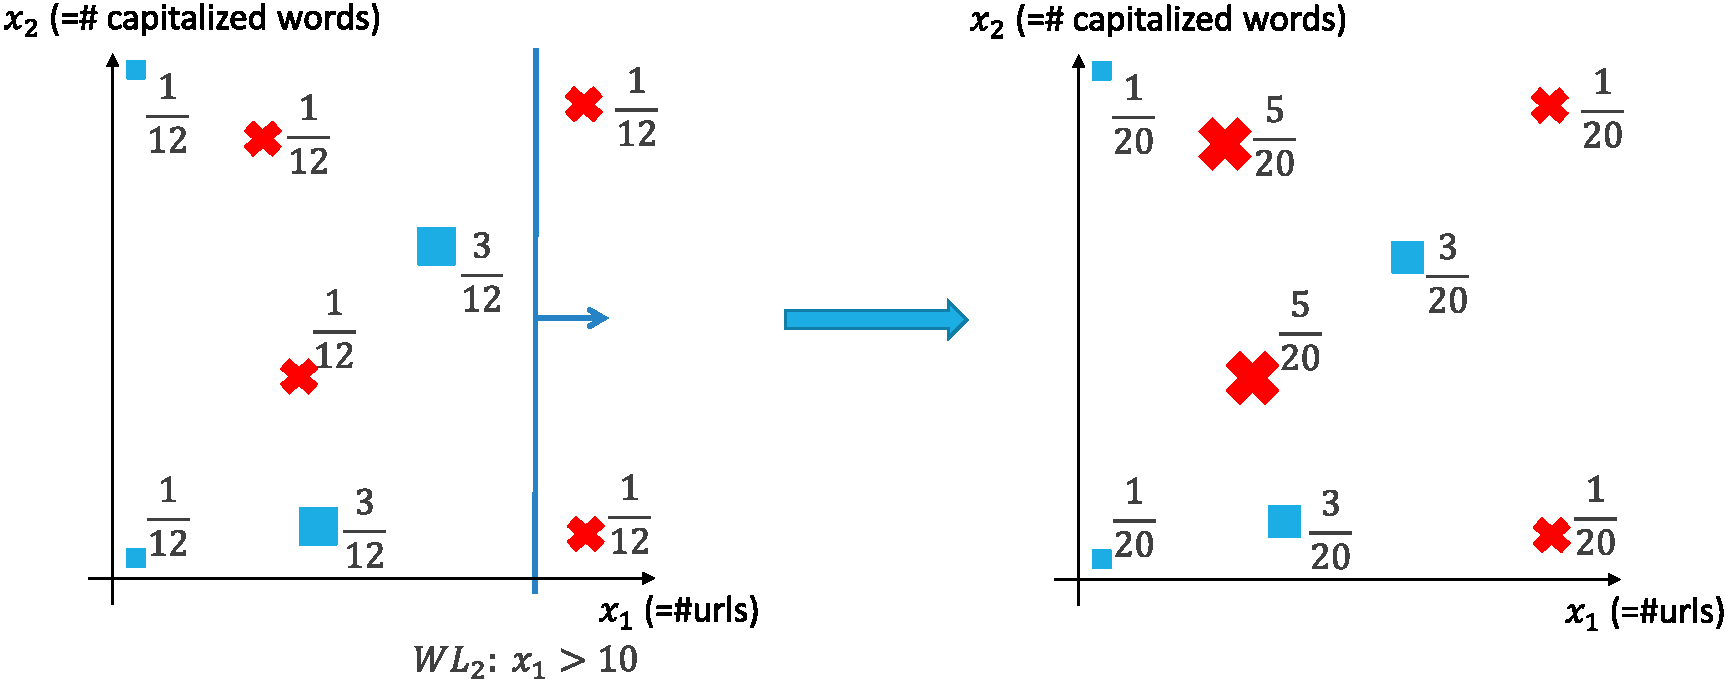
\includegraphics[width=0.7\linewidth]{./img/_adaboost_example3.pdf}
            \end{figure}

            Finally, the third classifier learns $x_2 > 20$. The error rate and reweigh factor are:
            \[ \varepsilon_3 = \frac{1}{20} + \frac{1}{20} + \frac{3}{20} \qquad
            \beta_3 = \frac{1 - \varepsilon_3}{\varepsilon_3} = 3 \]

            The strong classifier is defined as:
            \[ \texttt{SL}(x) = \begin{cases}
                1 & \text{if $\big( \ln(3)\texttt{WL}_1(x) + \ln(5)\texttt{WL}_2(x) + \ln(3)\texttt{WL}_3(x) \big) \geq 0$} \\
                -1 & \text{otherwise}
            \end{cases} \]
        \end{example}

    \item[Haar-like features] \marginnote{Haar-like features}
        For face detection, a $24 \times 24$ patch of the image is considered (for now) and the weak classifiers define rectangular filters composed of 2 to 4 subsections applied at fixed positions of the patch.

        Given a patch $x$, a weak learned $\texttt{WL}_j$ classifies it as:
        \[
            \texttt{WL}_j(x) = \begin{cases}
                1 & \text{if $s_j f_j \geq s_j \rho_j$} \\
                -1 & \text{otherwise}
            \end{cases}
        \]
        where the learned parameters are:
        \begin{itemize}
            \item The size and position of the filter ($f_j$ is the result of applying the filter).
            \item The polarity $s_j$.
            \item The threshold $\rho_j$.
        \end{itemize}

        \begin{figure}[H]
            \centering
            \begin{subfigure}{0.6\linewidth}
                \centering
                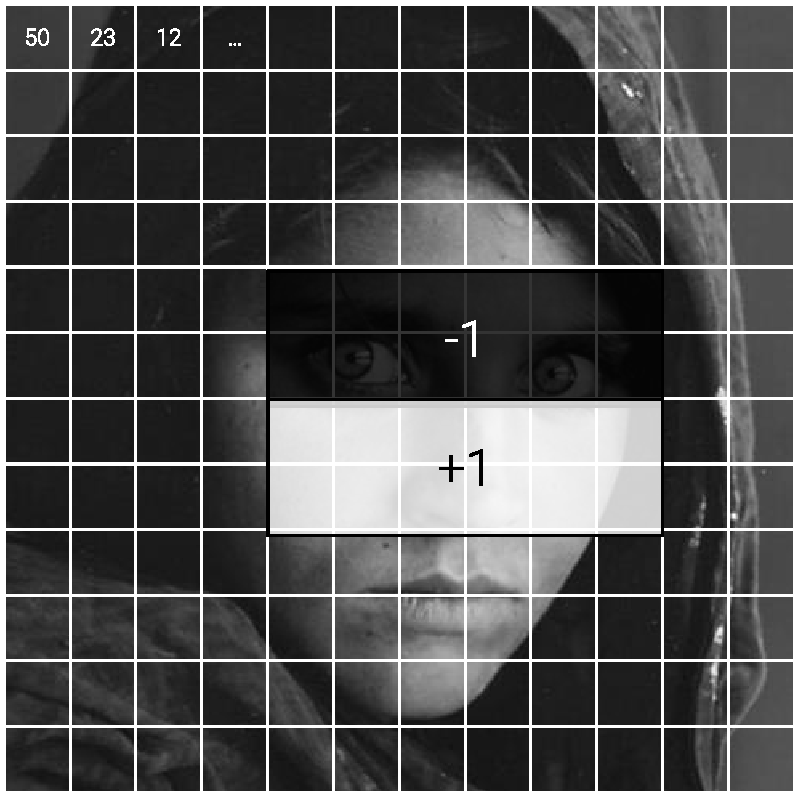
\includegraphics[width=0.5\linewidth]{./img/_haar_like_example.pdf}
                \caption{Filter applied on a patch}
            \end{subfigure}
            \hfill
            \begin{subfigure}{0.35\linewidth}
                \centering
                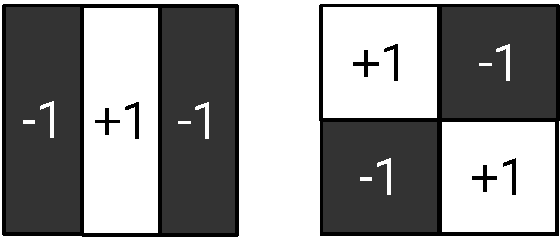
\includegraphics[width=0.65\linewidth]{./img/_haar_like_filters_example.pdf}
                \caption{Other possible filters}
            \end{subfigure}
            \caption{Example of filters}
        \end{figure}

        \begin{remark}
            AdaBoost is used to select a subset of the most effective filters.
        \end{remark}
\end{description}


\subsection{Integral images}

\begin{description}
    \item[Integral image] \marginnote{Integral image}
        Given an image $I$, its corresponding integral image $II$ is defined as:
        \[ II(i, j) = \sum_{i' \leq i, j' \leq j} I(i', j') \]
        In other words, the value at coordinates $(i, j)$ in the integral image is the sum of all the pixels of the original image in an area that starts from the top-left corner and has as bottom-right corner the pixel at $(i, j)$.
        \begin{figure}[H]
            \centering
            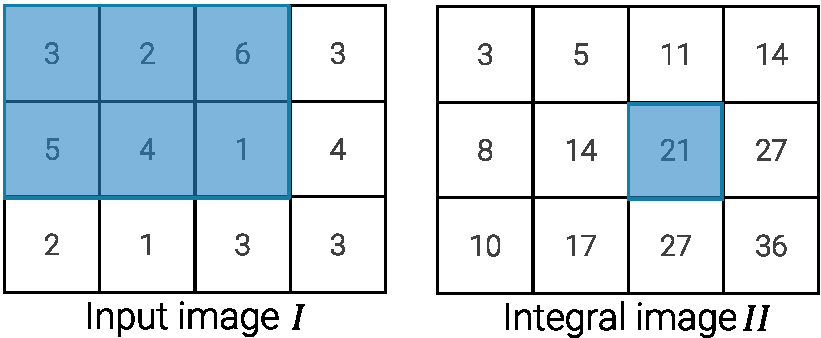
\includegraphics[width=0.45\linewidth]{./img/_integral_image.pdf}
            \caption{Example of integral image}
        \end{figure}

        \begin{remark}
            In practice, the integral image can be computed recursively as:
            \[ II(i, j) = II(i, j-1) + II(i-1, j) - II(i-1, j-1) + I(i, j) \]
        \end{remark}

    \item[Fast feature computation] \marginnote{Fast feature computation}
        Given an image $I$ and its integral image $II$, the sum of the pixels in a rectangular area of $I$ can be computed in constant time as:
        \[ II(A) - II(B) - II(C) + II(D) \]
        where $A$, $B$, $C$, and $D$ are coordinates defined as in \Cref{fig:integral_image_features}.
        \begin{figure}[H]
            \centering
            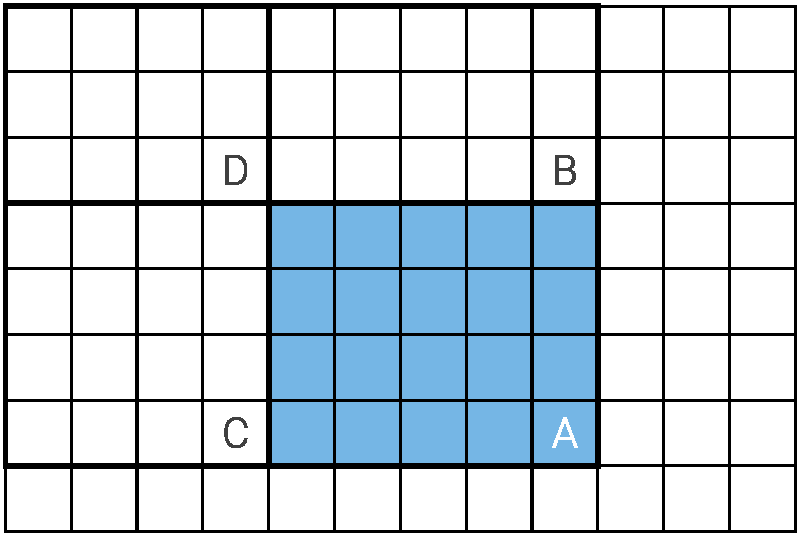
\includegraphics[width=0.5\linewidth]{./img/_integral_image_feature.pdf}
            \caption{Summation of the pixels in the blue area}
            \label{fig:integral_image_features}
        \end{figure}

    \item[Multi-scale sliding window] \marginnote{Multi-scale sliding window}
        During inference, Viola-Jones is a sliding window detector that scans the image considering patches of fixed size.

        To achieve scale-invariance, patches of different size are used, scaling the rectangular filters accordingly.

        \begin{remark}
            The integral image allows to compute the features in constant time independently of the patch size.
        \end{remark}
\end{description}


\subsection{Cascade}

\begin{description}
    \item[Cascade] \marginnote{Cascade}
        To obtain real-time predictions, a hierarchy of classifiers is used to quickly reject background patches. The first classifier considers a few features while the following ones use more.

        \begin{remark}
            The simpler classifiers have a high recall so that they do not discard faces.
        \end{remark}

        \begin{figure}[H]
            \centering
            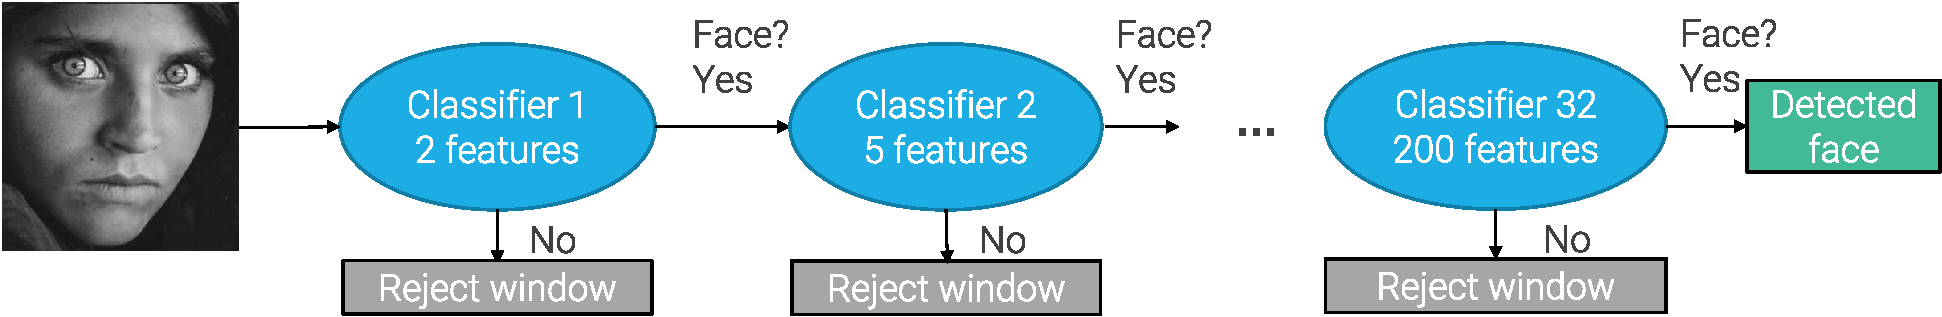
\includegraphics[width=0.8\linewidth]{./img/_viola_jones_cascade.pdf}
        \end{figure}
\end{description}


\subsection{Non-maximum suppression}

\begin{description}
    \item[Non-maximum suppression (NMS)] \marginnote{Non-maximum suppression (NMS)}
        Algorithm to obtain a single bounding box from several overlapping ones. Given the set of all the bounding boxes with their confidence that a detector found, NMS works as follows:
        \begin{enumerate}
            \item Until there are unchecked boxes:
            \begin{enumerate}
                \item Consider the bounding box with the highest confidence.
                \item Eliminate all boxes with overlap higher than a chosen threshold (e.g., $\texttt{IoU} > 0.5$).
            \end{enumerate}
        \end{enumerate}

        \begin{remark}
            If two objects are close, NMS might detect them as a single instance.
        \end{remark}
\end{description}



\section{CNN for object detection}


\subsection{Object localization}

\begin{description}
    \item[Object localization] \marginnote{Object localization}
        Subset of object detection problems where it is assumed that there is only a single object to detect.

    \item[CNN for object localization] \marginnote{CNN for object localization}
        A pre-trained CNN can be used as feature extractor with two heads:
        \begin{descriptionlist}
            \item[Classification head] Used to determine the class.
            \item[Regression head] Used to determine the bounding box.
        \end{descriptionlist}

        Given:
        \begin{itemize}
            \item The ground-truth class $c^{(i)}$ and bounding box $BB^{(i)}$,
            \item The predicted class logits $\texttt{scores}^{(i)}$ and bounding box $\widehat{BB}^{(i)}$,
        \end{itemize} 
        training is a multi-task learning problem with two losses:
        \[ \mathcal{L}^{(i)} = \mathcal{L}_\text{CE}\left( \texttt{softmax}(\texttt{scores}^{(i)}), \mathbbm{1}[c^{(i)}] \right) + \lambda \mathcal{L}_\text{MSE}\left(\widehat{BB}^{(i)}, BB^{(i)} \right) \]

        \begin{figure}[H]
            \centering
            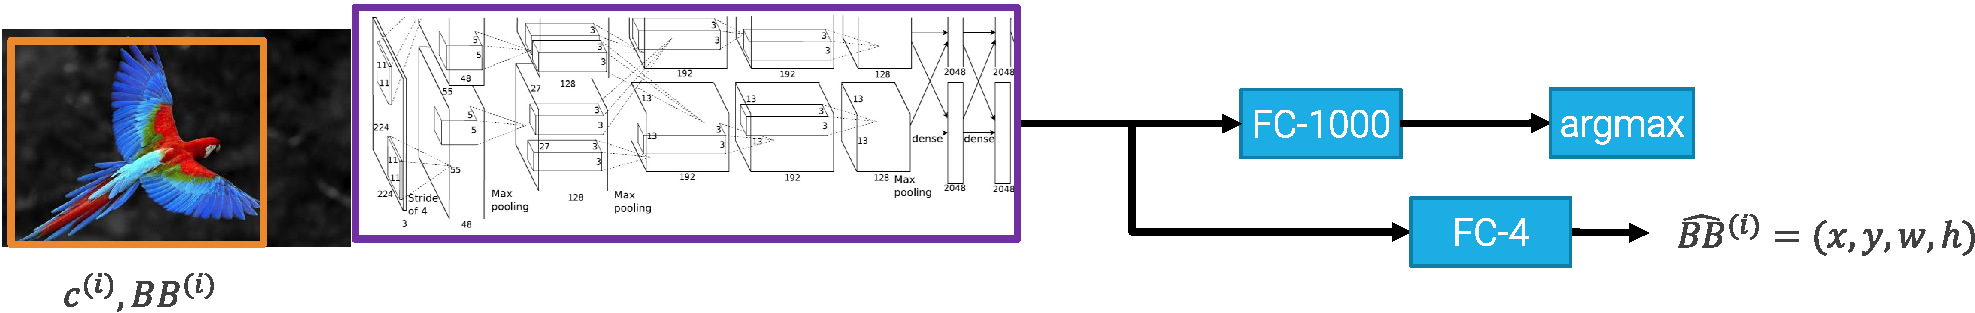
\includegraphics[width=0.9\linewidth]{./img/_cnn_object_localization.pdf}
            \caption{Localizer with AlexNet as feature extractor and 1000 classes}
        \end{figure}

        \begin{remark}
            A localization CNN can be used as a sliding window detector to detect multiple objects.

            An additional background class (\texttt{bg}) has to be added to mark patches without an object. Moreover, when a patch belongs to the background, the loss related to the bounding box should be ignored. Therefore, the loss becomes:
            \[ \mathcal{L}^{(i)} = \mathcal{L}_\text{CE}\left( \texttt{softmax}(\texttt{scores}^{(i)}), \mathbbm{1}[c^{(i)}] \right) + \lambda \mathbbm{1}[c^{(i)} \neq \texttt{bg}] \mathcal{L}_\text{MSE}\left(\widehat{BB}^{(i)}, BB^{(i)} \right) \]
            where $\mathbbm{1}[c^{(i)} \neq \texttt{bg}]$ is $1$ iff the ground-truth class $c^{(i)}$ is not the background class.

            This approach has two main problems:
            \begin{itemize}
                \item Background patches are usually more frequent, requiring additional work to balance the dataset or mini-batch.
                \item There are too many patches to check.
            \end{itemize}
        \end{remark}
\end{description}


\subsection{Region proposal}

\begin{description}
    \item[Region proposal] \marginnote{Region proposal}
        Class of algorithms to find regions likely to contain an object.

        \begin{description}
            \item[Selective search] \marginnote{Selective search}
            Region proposal algorithm that works as follows:
            \begin{enumerate}
                \item Segment the image into superpixels (i.e., uniform regions).
                \item Merge superpixels based on similarity of color, texture, or size. Each aggregation generates a proposed region.
                \item Repeat until everything collapses in a single region.
            \end{enumerate}
        \end{description}

        \begin{remark}
            Region proposal algorithms should have a high recall.
        \end{remark}

        \begin{figure}[H]
            \centering
            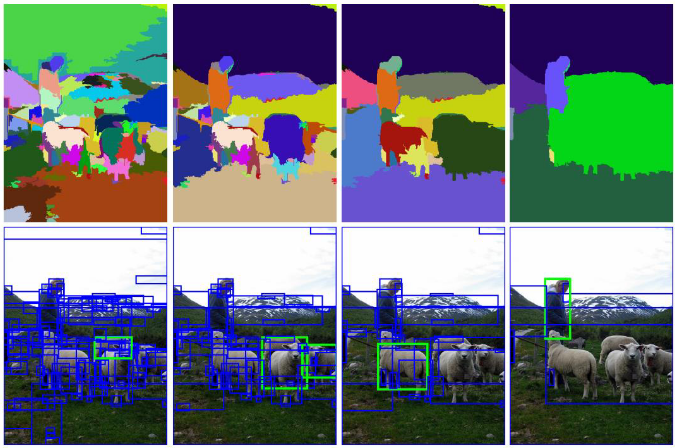
\includegraphics[width=0.45\linewidth]{./img/selective_search.png}
            \caption{Example of some iterations of selective search}
        \end{figure}

    \item[Region-based CNN (R-CNN)] \marginnote{Region-based CNN (R-CNN)}
        Use a CNN for object localization with selective search. The workflow is the following:
        \begin{enumerate}
            \item Run selective search to get the proposals.
            \item For each proposal:
            \begin{enumerate}
                \item Warp the proposed crop to the input shape of the CNN.
                \item Feed the warped crop to the CNN to get:
                \begin{itemize}
                    \item A class prediction.
                    \item A bounding box correction (as selective search already gives a box).
                \end{itemize}
            \end{enumerate}
        \end{enumerate}

        \begin{figure}[H]
            \centering
            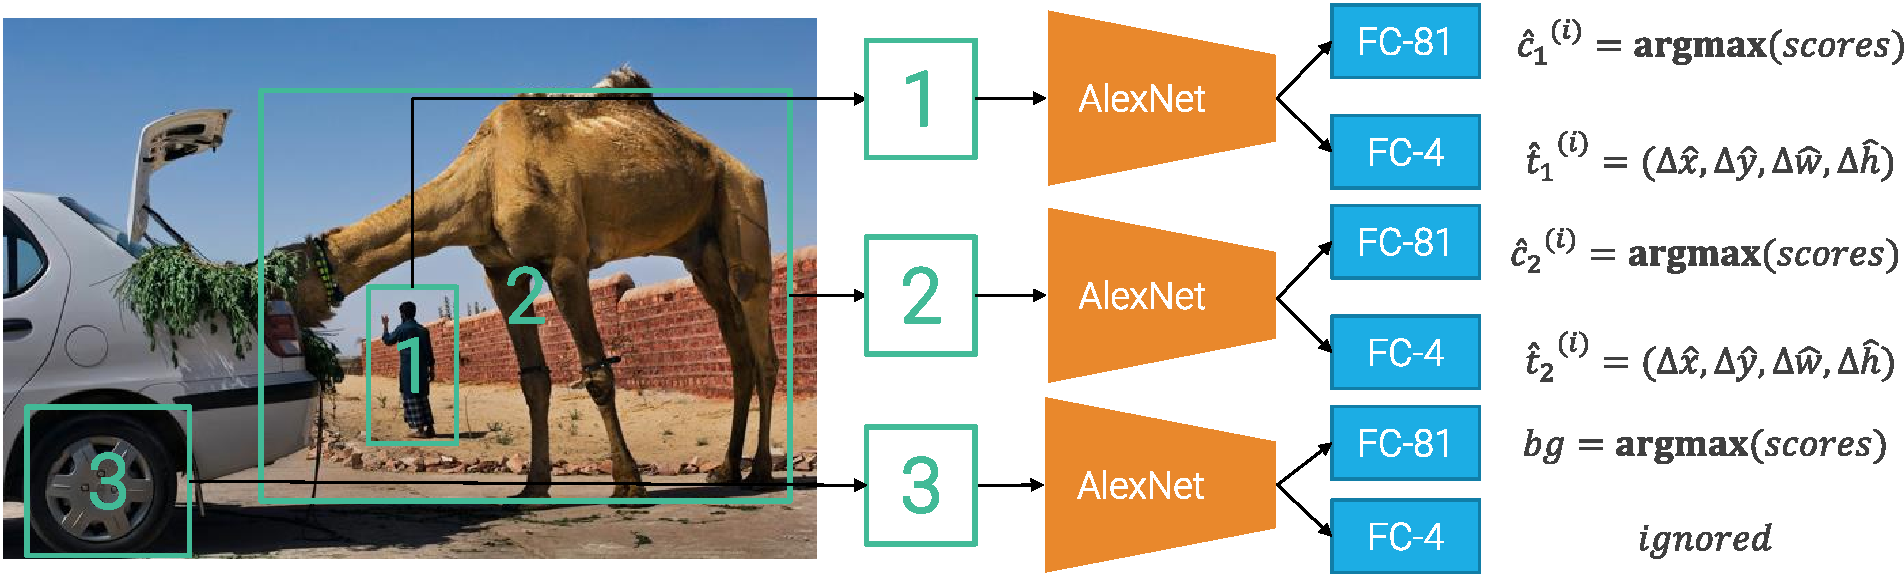
\includegraphics[width=0.8\linewidth]{./img/_r_cnn.pdf}
            \caption{Example of R-CNN using AlexNet}
        \end{figure}

        \begin{description}
            \item[Bounding box correction] \marginnote{Bounding box correction}
                Given a selective search bounding box $BB_{\text{SS}}$ and the network predicted correction $\hat{t}$:
                \[ 
                    BB_{\text{SS}} = (x_{\text{SS}}, y_{\text{SS}}, w_{\text{SS}}, h_{\text{SS}})
                    \qquad
                    \hat{t} = (\Delta\hat{x}, \Delta\hat{y}, \Delta\hat{w}, \Delta\hat{h})
                \]
                the output box $BB_{\text{out}}$ is given by:
                \[ 
                    BB_{\text{out}} = ( 
                        x_{\text{SS}} + w_{\text{SS}}\Delta\hat{x},
                        y_{\text{SS}} + h_{\text{SS}}\Delta\hat{y},
                        w_{\text{SS}} \exp(\Delta\hat{w}),
                        h_{\text{SS}} \exp(\Delta\hat{h})
                    ) 
                \]
                where the center is a translation relative to the box size and the dimensions are log-space scaled.

                \begin{remark}
                    This formulation is due to the fact that a neural network tend to output smaller values, so overall it results an easier task to learn.
                \end{remark}

                \begin{description}
                    \item[Training] 
                    Given a training sample $x^{(i)}$ with class $c^{(i)}$ and bounding box $BB^{(i)} = [x_\text{GT}, y_\text{GT}, w_\text{GT}, h_\text{GT}]$, the selective search box $BB_\text{SS}^{(i)}$ associated to it during training is the one with the most overlap, while the others are considered background. The target correction $t^{(i)} = [\Delta x, \Delta y, \Delta w, \Delta h]$ is computed as:
                    \[ 
                        \Delta x = \frac{x_\text{GT} - x_\text{SS}}{w_\text{SS}}
                        \quad
                        \Delta y = \frac{y_\text{GT} - y_\text{SS}}{h_\text{SS}}
                        \quad
                        \Delta w = \ln\left(\frac{w_\text{GT}}{w_\text{SS}} \right)
                        \quad
                        \Delta w = \ln\left( \frac{h_\text{GT}}{h_\text{SS}} \right)
                    \]
                    The loss is then defined as:
                    \[ \mathcal{L}^{(i)} = \mathcal{L}_\text{CE}\left( \texttt{softmax}(\texttt{scores}^{(i)}), \mathbbm{1}[c^{(i)}] \right) + \lambda \mathbbm{1}[c^{(i)} \neq \texttt{bg}] \mathcal{L}_\text{MSE}\left(\widehat{t}^{(i)}, t^{(i)} \right) \]

                \end{description}
        \end{description}

        \begin{remark}
            Empirically, it has been observed that feature computation, fine-tuning, bounding box correction, and architecture are important to increase mAP.
        \end{remark}

        \begin{remark}
            Instead of AlexNet, any other CNN can potentially be used.
        \end{remark}

        \begin{remark}
            R-CNN is slow as it requires to process each proposed crop.
        \end{remark}

    \item[Fast R-CNN] \marginnote{Fast R-CNN}
        Optimization to R-CNNs that avoids processing overlapping pixels of the proposed crops with the CNN multiple times:
        \begin{enumerate}
            \item Process the original image with the feature extractor section of the CNN.
            \item Compute the proposed crops from the feature extractor activations and adjust to the correct shapes through pooling.
            \item Feed each crop to the remaining fully-connected layers of the CNN and the task-specific heads.
        \end{enumerate}

        \begin{figure}[H]
            \centering
            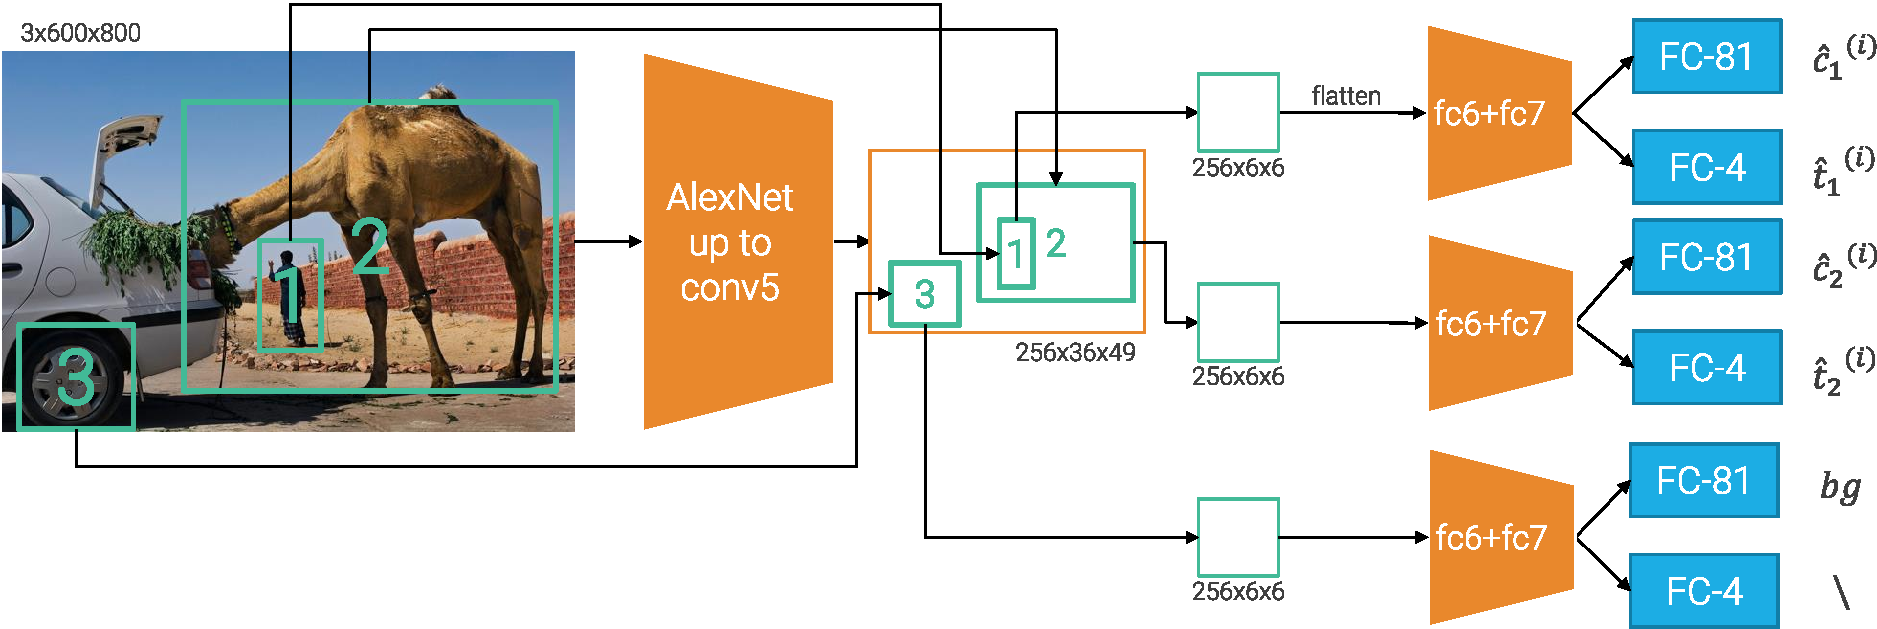
\includegraphics[width=0.8\linewidth]{./img/_fast_r_cnn.pdf}
            \caption{Example of fast R-CNN using AlexNet}
        \end{figure}

        \begin{description}
            \item[Region of interest pool (RoIPool)] \marginnote{Region of interest pool (RoIPool)}
                Given an input activation of shape $C_a \times H_a \times W_a$ and the desired output spatial dimension $H_o \times W_o$, RoIPool allows to obtain an output of shape $C_a \times H_o \times W_o$ as follows:
                \begin{enumerate}
                    \item Project the proposed region from the original image to the feature extractor activations.
                    \item Snap the projection to grid (i.e., apply rounding).
                        \begin{remark}
                            As a single pixel in the activation encodes multiple pixels of the input image, snapping might lose some information.
                        \end{remark}
                        \begin{figure}[H]
                            \raggedleft
                            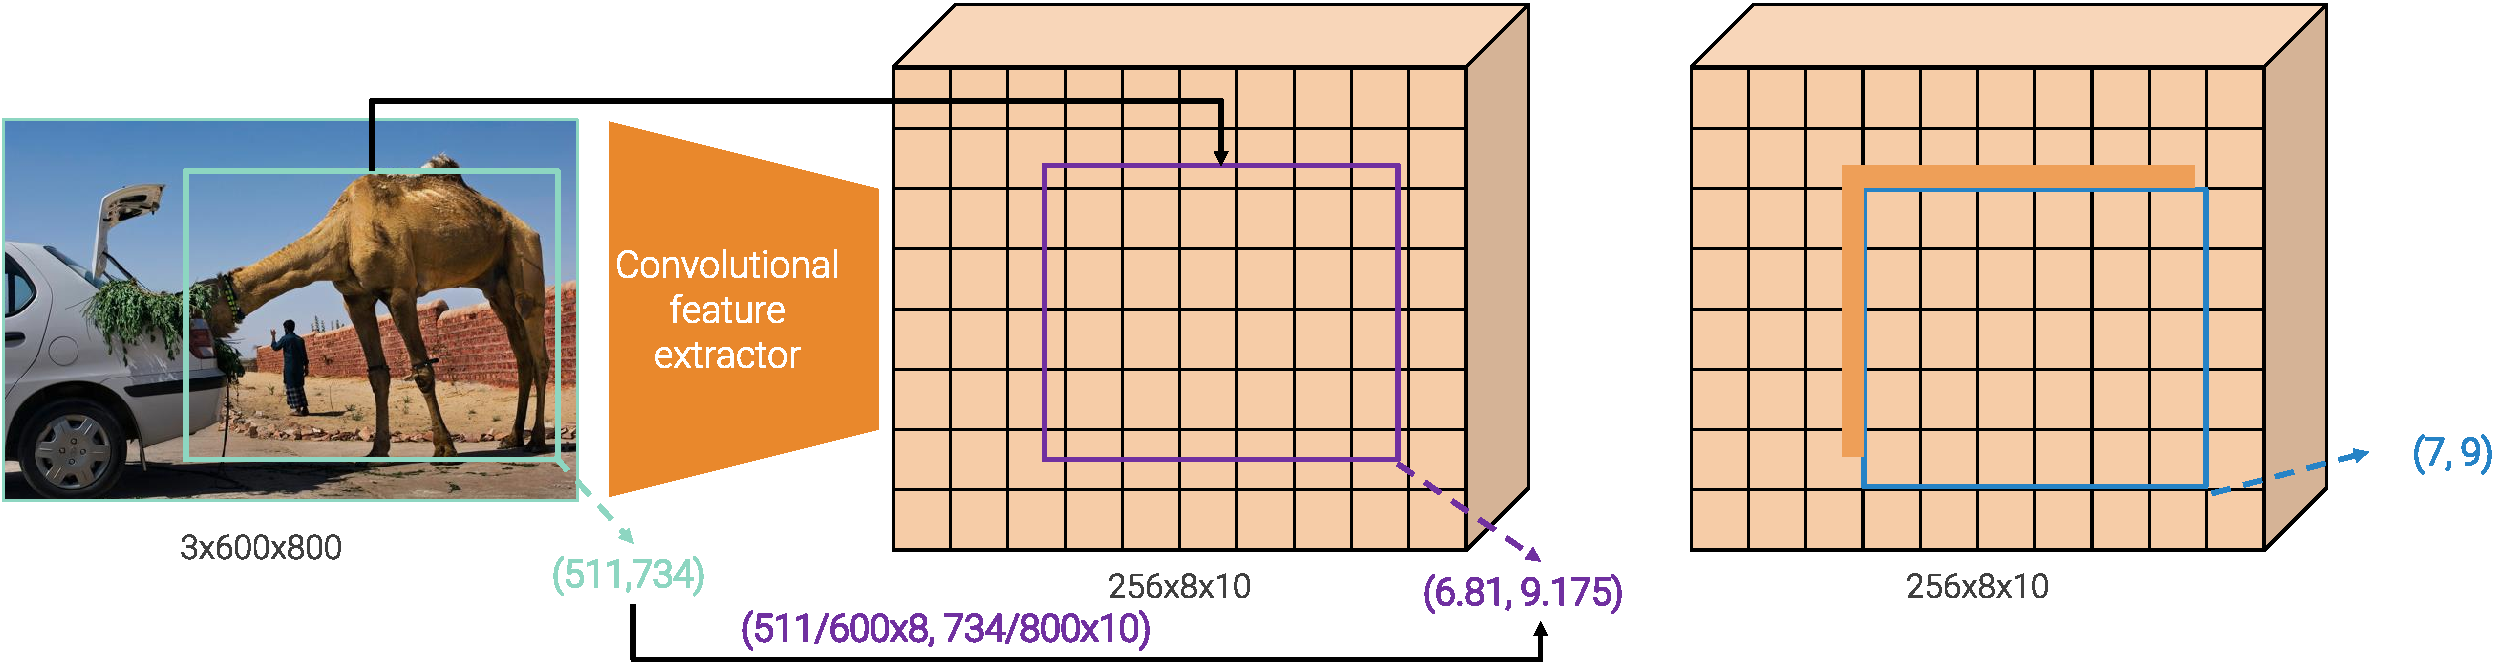
\includegraphics[width=0.85\linewidth]{./img/_roipool_snap.pdf}
                            \caption{Project and snap operations}
                        \end{figure}
                    \item Apply max pooling with kernel of approximately size $\left\lceil \frac{H_r}{H_O} \right\rceil \times \left\lceil \frac{W_r}{W_O} \right\rceil$ and stride approximately $\left\lfloor \frac{H_r}{H_O} \right\rfloor \times \left\lfloor \frac{W_r}{W_O} \right\rfloor$.
                        \begin{remark}
                            Approximations are needed as the spatial dimension of the crop might not be directly convertible to the desired output shape. So, some iterations might not use the precise kernel size or stride.
                        \end{remark}
                        \begin{figure}[H]
                            \raggedleft
                            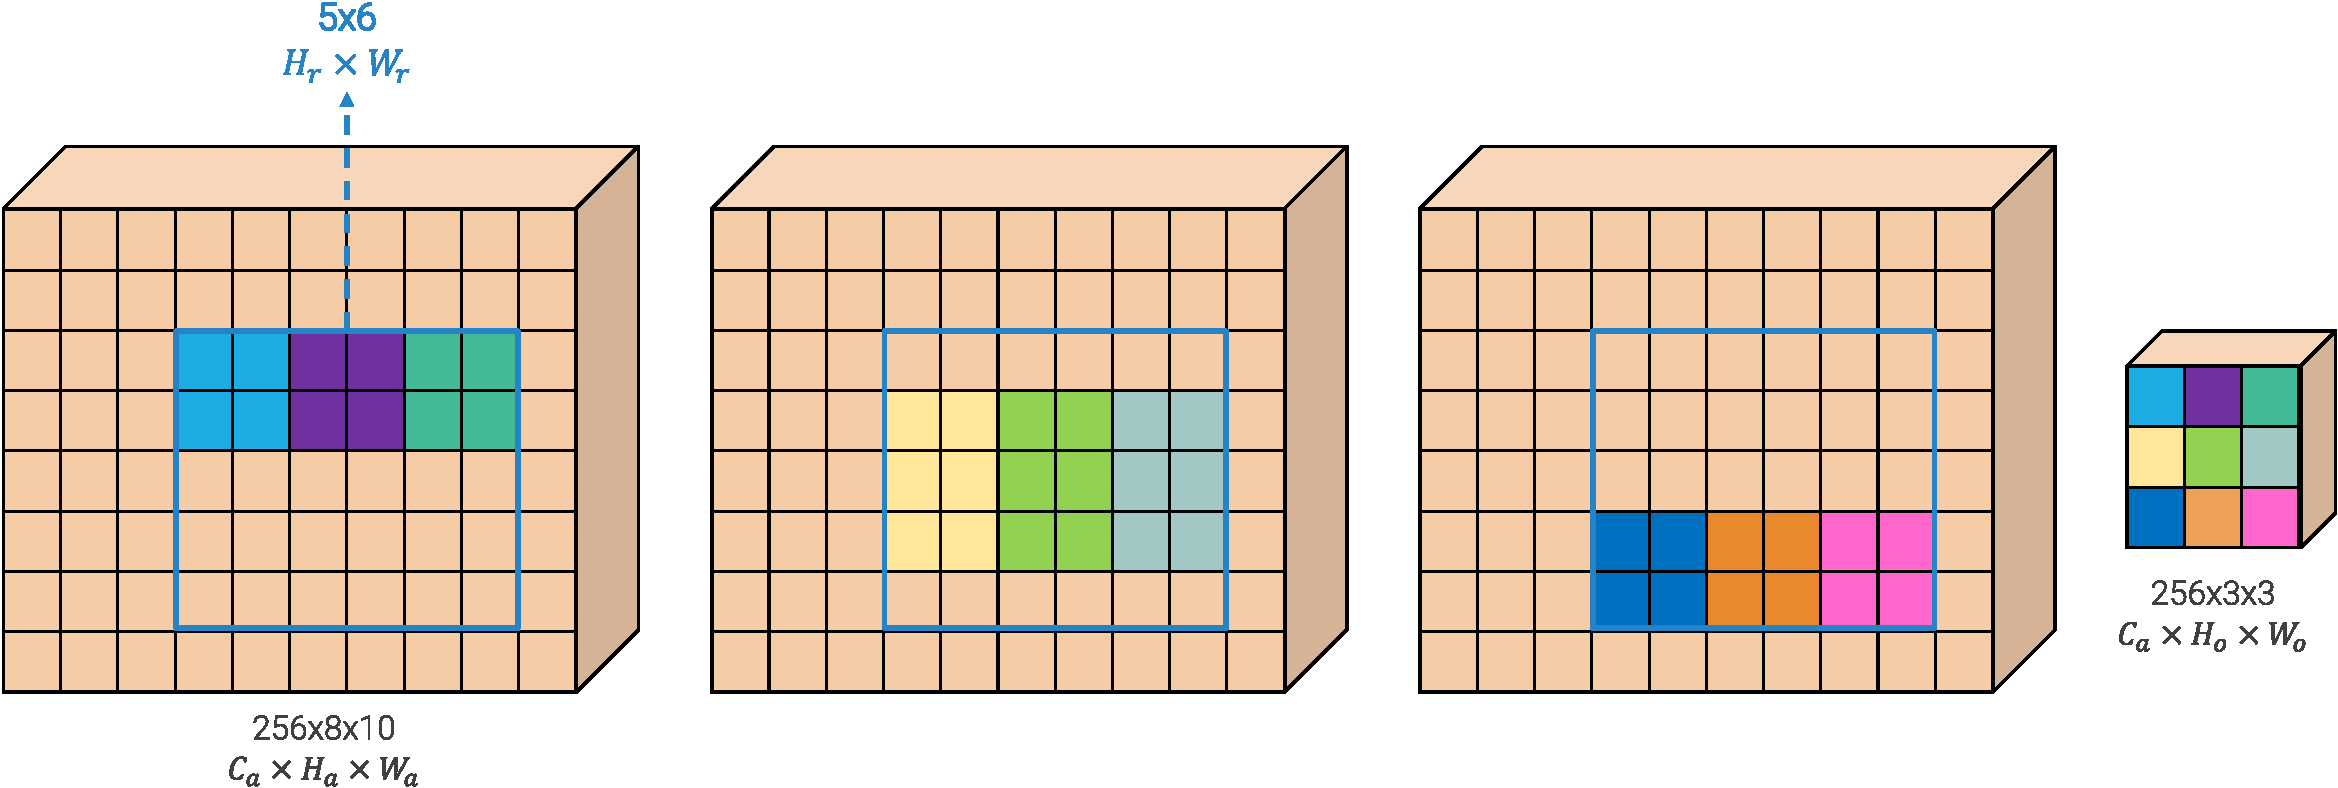
\includegraphics[width=0.85\linewidth]{./img/_roipool_maxpool.pdf}
                            \caption{Pooling operation with varying kernel size}
                        \end{figure}
                \end{enumerate}

                \begin{remark}
                    Snapping and approximate pooling introduce two sources of quantization.
                \end{remark}

            \item[Huber loss] \marginnote{Huber loss}
                Instead of L2, fast R-CNN uses the Huber (i.e., smooth L1) loss to compare bounding boxes:
                \[ 
                    \begin{gathered}
                        \mathcal{L}_{BB}^{(i)} = \sum_{d \in \{ x, y, w, h \}} \mathcal{L}_\text{huber}\left( \Delta\hat{d}^{(i)} - \Delta d^{(i)} \right) \\
                        \mathcal{L}_\text{huber}(a) = \begin{cases}
                            \frac{1}{2}a^2 & \text{if $|a| \leq 1$} \\
                            |a| - \frac{1}{2} & \text{otherwise}
                        \end{cases}
                    \end{gathered}
                \]

                \begin{remark}
                    L2 grows quadratically with the loss which makes it sensitive to outliers. Smooth L1 maintains the gradient constant to $1$ for big values.
                \end{remark}
        \end{description}

        \begin{remark}
            Fast R-CNN reduces the number of FLOPs when applying the convolutions but moves the bottleneck to the feed-forward layers.
            \begin{table}[H]
                \centering
                \footnotesize
                \begin{tabular}{rcc}
                    \toprule
                    & \textbf{Conv FLOPs} & \textbf{FF FLOPs} \\
                    \midrule
                    \textbf{R-CNN} & $n \cdot 2154$ M & $n \cdot 117$ M \\
                    \textbf{Fast R-CNN} & $\num{16310}$ M & $n \cdot 117$ M \\
                    \bottomrule
                \end{tabular}
                \caption{FLOPs comparison with AlexNet as CNN and $n$ proposals}
            \end{table}
        \end{remark}

        \begin{remark}
            The slowest component of fast R-CNN is selective search.
        \end{remark}

    \item[Faster R-CNN] \marginnote{Faster R-CNN}
        Selective search is dropped and a region proposal network (RPN) is used:
        \begin{enumerate}
            \item Pass the input image through the feature extractor section of the CNN.
            \item Feed the activations to the RPN to determine the regions of interest.
            \item Continue as in fast R-CNN.
        \end{enumerate}

        \begin{figure}[H]
            \centering
            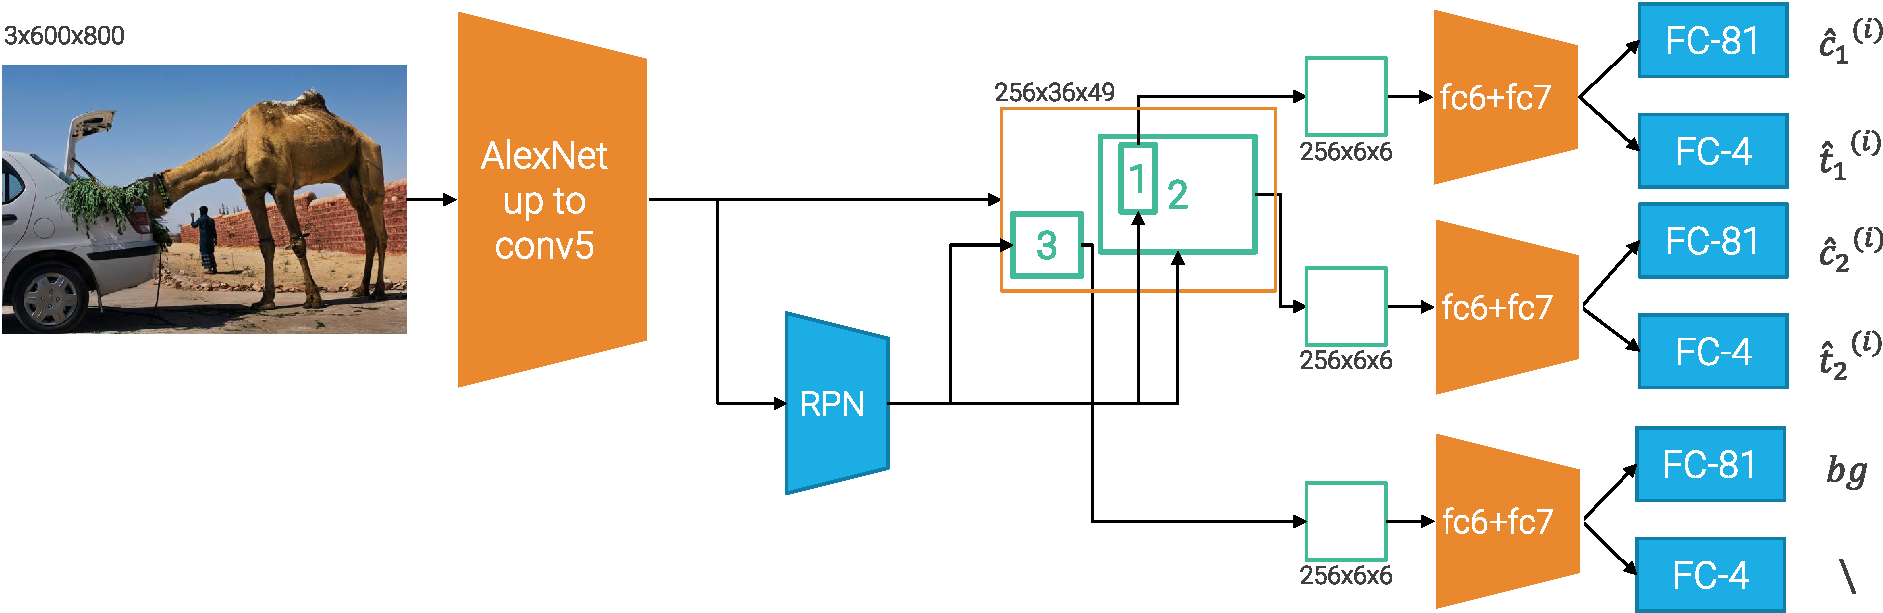
\includegraphics[width=0.8\linewidth]{./img/_faster_r_cnn.pdf}
            \caption{Example of faster R-CNN using AlexNet}
        \end{figure}

        \begin{description}
            \item[Region proposal network (RPN)] \marginnote{Region proposal network (RPN)}
            Network that takes as input the image activations of shape $C_L \times H_L \times W_L$ and outputs:
            \begin{itemize}
                \item The objectness scores of shape $2 \times H_L \times W_L$.
                    \begin{remark}
                        The two channels are due to the fact that the original paper uses a two-way softmax, which in practice is equivalent to a sigmoid.
                    \end{remark}
                \item The proposed boxes of shape $4 \times H_L \times W_L$.
            \end{itemize}
            In other words, an RPN makes a prediction at each input pixel.

            \begin{remark}
                RPN has a small fixed receptive field (that should roughly be the size of an object), but can  predict boxes larger than it.
            \end{remark}

            \begin{remark}
                As is, RPN is basically solving object detection as it has to determine the exact box for the objects, which might be a difficult task.
            \end{remark}

            \begin{description}
                \item[Anchor] \marginnote{Anchor}
                    Known bounding box with fixed scale and aspect-ratio.

                \begin{description}
                    \item[Anchor correction] \marginnote{Anchor correction}
                        Make an RPN predict a correction for a known anchor whose center is positioned at the center of the receptive field.

                        \begin{figure}[H]
                            \raggedleft
                            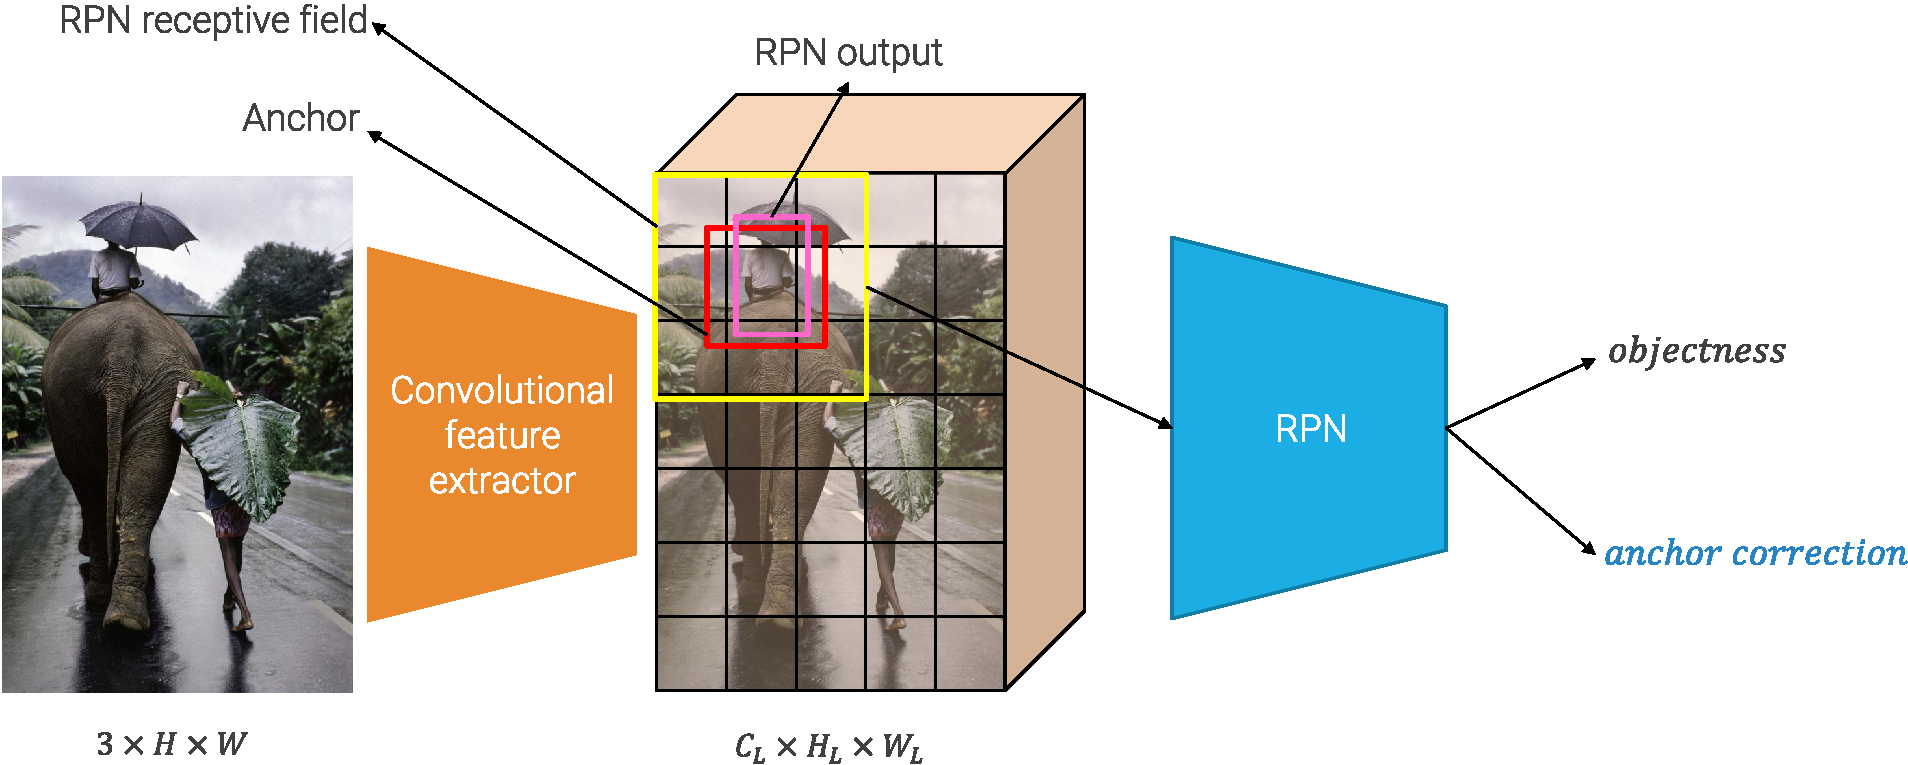
\includegraphics[width=0.8\linewidth]{./img/_rpn_anchor.pdf}
                            \caption{Example of an iteration of a 1-anchor RPN}
                        \end{figure}

                    \item[$\mathbf{k}$ anchors correction] \marginnote{$k$ anchors correction}
                        Consider $k$ different anchors so that the RPN outputs $k$ objectness scores (overall shape of $2k \times H_L \times W_L$) and $k$ corrections (overall shape of $4k \times H_L \times W_L$) at each pixel.

                        \begin{remark}
                            Virtually, this can be seen as putting together the outputs of $k$ different $1$-anchor RPN (with different anchors).
                        \end{remark}
                \end{description}

                \item[Architecture]
                    An RPN is implemented as a two-layer CNN:
                    \begin{enumerate}
                        \item A $3 \times 3$ convolution with padding $1$, stride $0$, $256$ output channels, and ReLU as activation.
                        \item Two parallel $1 \times 1$ convolutions with no padding and stride $1$ with $2k$ and $4k$ output channels, respectively.
                    \end{enumerate}
                    \begin{figure}[H]
                        \raggedleft
                        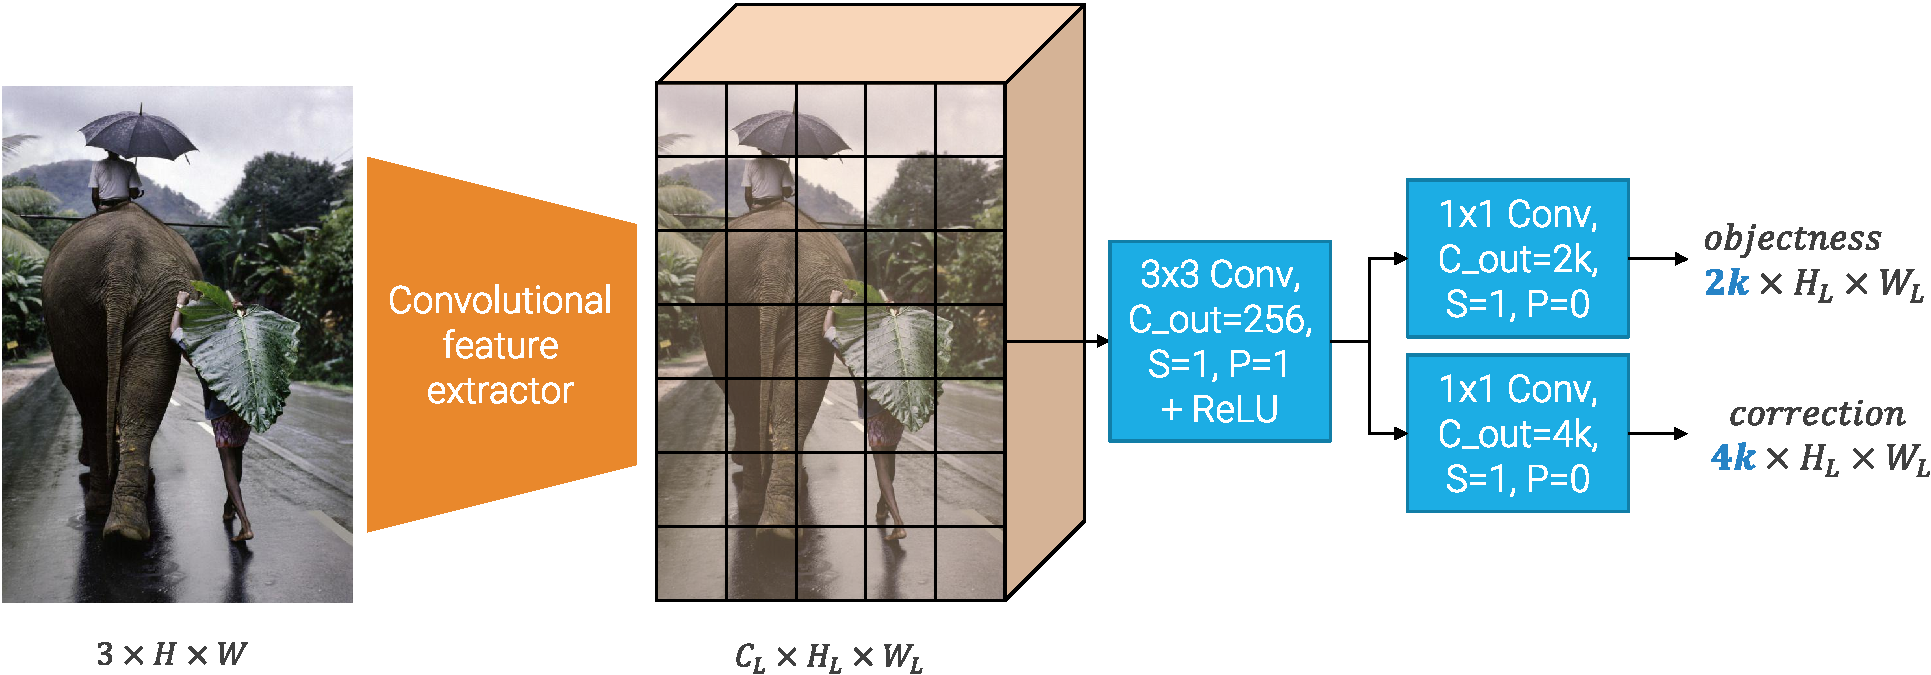
\includegraphics[width=0.7\linewidth]{./img/_rpn_architecture.pdf}
                    \end{figure}
            \end{description}

            \begin{remark}
                Only the proposals with the highest objectness scores are considered at training and test time.
            \end{remark}

            \begin{description}
                \item[Training]
                    Given a training image $x^{(i)}$ and a bounding box $BB_\text{GT}$, the $j$-th anchor $BB_A$ can be a:
                    \begin{descriptionlist}
                        \item[Negative anchor] 
                            $BB_A$ has objectness score $o^{(i, j)} = 0$ (i.e., it contains background) if $\texttt{IoU}(BB_{GT}, BB_A) < 0.3$.
                        \item[Positive anchor] 
                            $BB_A$ has objectness score $o^{(i, j)} = 1$ (i.e., it contains an object) whether:
                            \begin{itemize}
                                \item $\texttt{IoU}(BB_{GT}, BB_A) \geq 0.7$.
                                \item $\texttt{IoU}(BB_{GT}, BB_A)$ is the largest and none of the others are $\geq 0.7$.
                            \end{itemize}
                        \item[Ignored anchor] 
                            $BB_A$ is not considered for this sample in all other cases.
                    \end{descriptionlist}

                    A mini-batch is composed of all the positive anchors and it is filled with negative anchors to reach the desired size.

                    \begin{remark}
                        Differently from R-CNN, multiple boxes have a positive label as it is ambiguous to determine which anchor is responsible for recognizing a particular object.
                    \end{remark}
            \end{description}
        \end{description}
\end{description} 

\begin{remark}
    R-CNN is unable to detect objects smaller than the grid size.
\end{remark}


\subsection{Multi-scale detection}

\begin{description}
    \item[Image pyramid multi-scale detection] \marginnote{Image pyramid multi-scale detection}
        Obtain a feature pyramid by feeding the input image to the convolutional feature extractor at different scales.

        \begin{remark}
            This approach creates effective features at different scales, but it is computationally expensive.
        \end{remark}

        \begin{figure}[H]
            \centering
            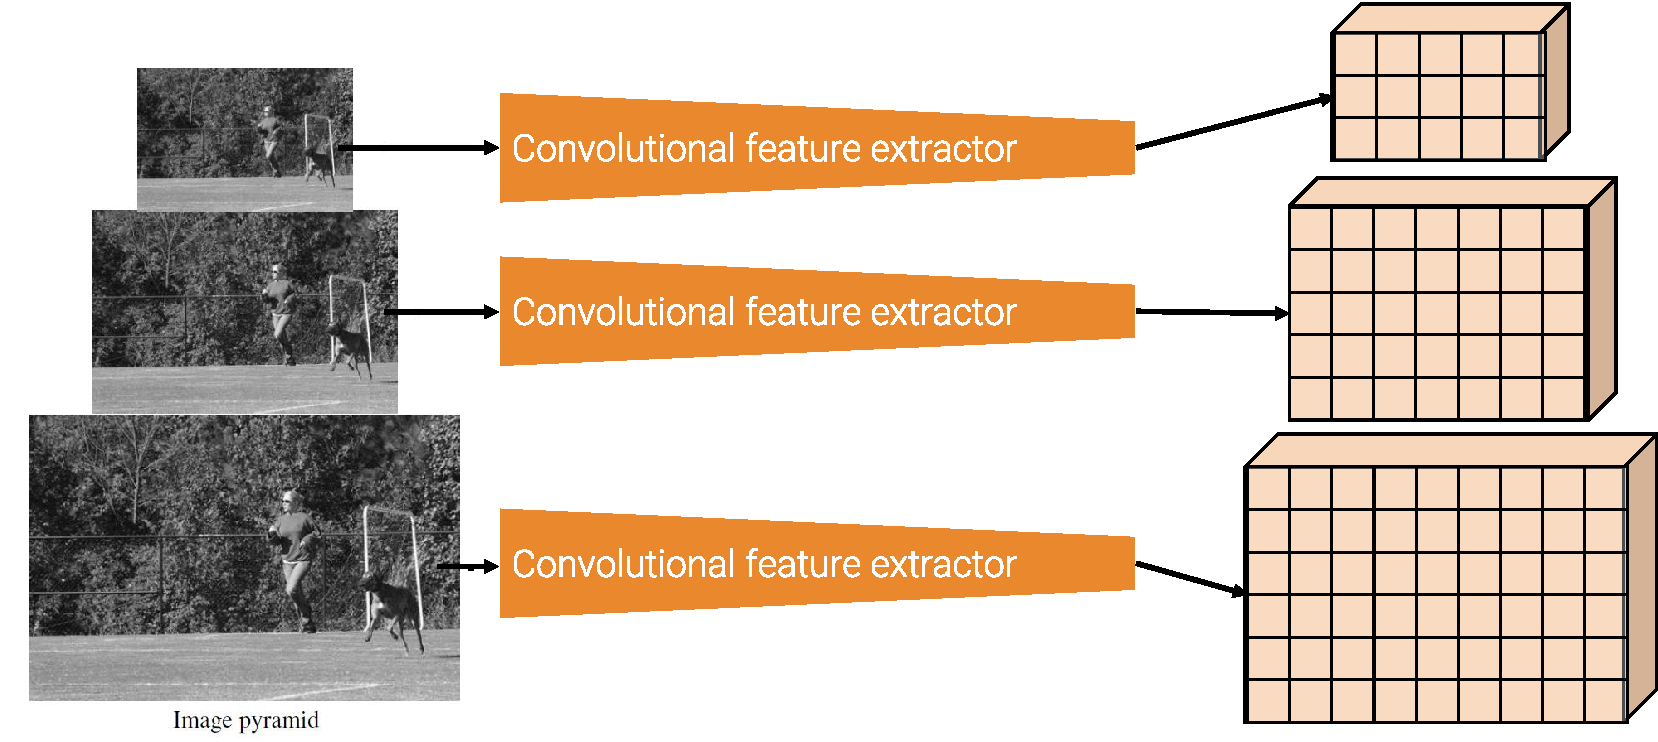
\includegraphics[width=0.6\linewidth]{./img/_image_pyramid_multi_scale.pdf}
        \end{figure}

    \item[CNN pyramid multi-scale detection] \marginnote{CNN pyramid multi-scale detection}
        CNNs naturally produce a pyramid of features composed of the activations at each stage.

        \begin{remark}
            This approach do not affect computational cost, but features at smaller scales have bad semantic quality as they are at the beginning of the network.
        \end{remark}

        \begin{figure}[H]
            \centering
            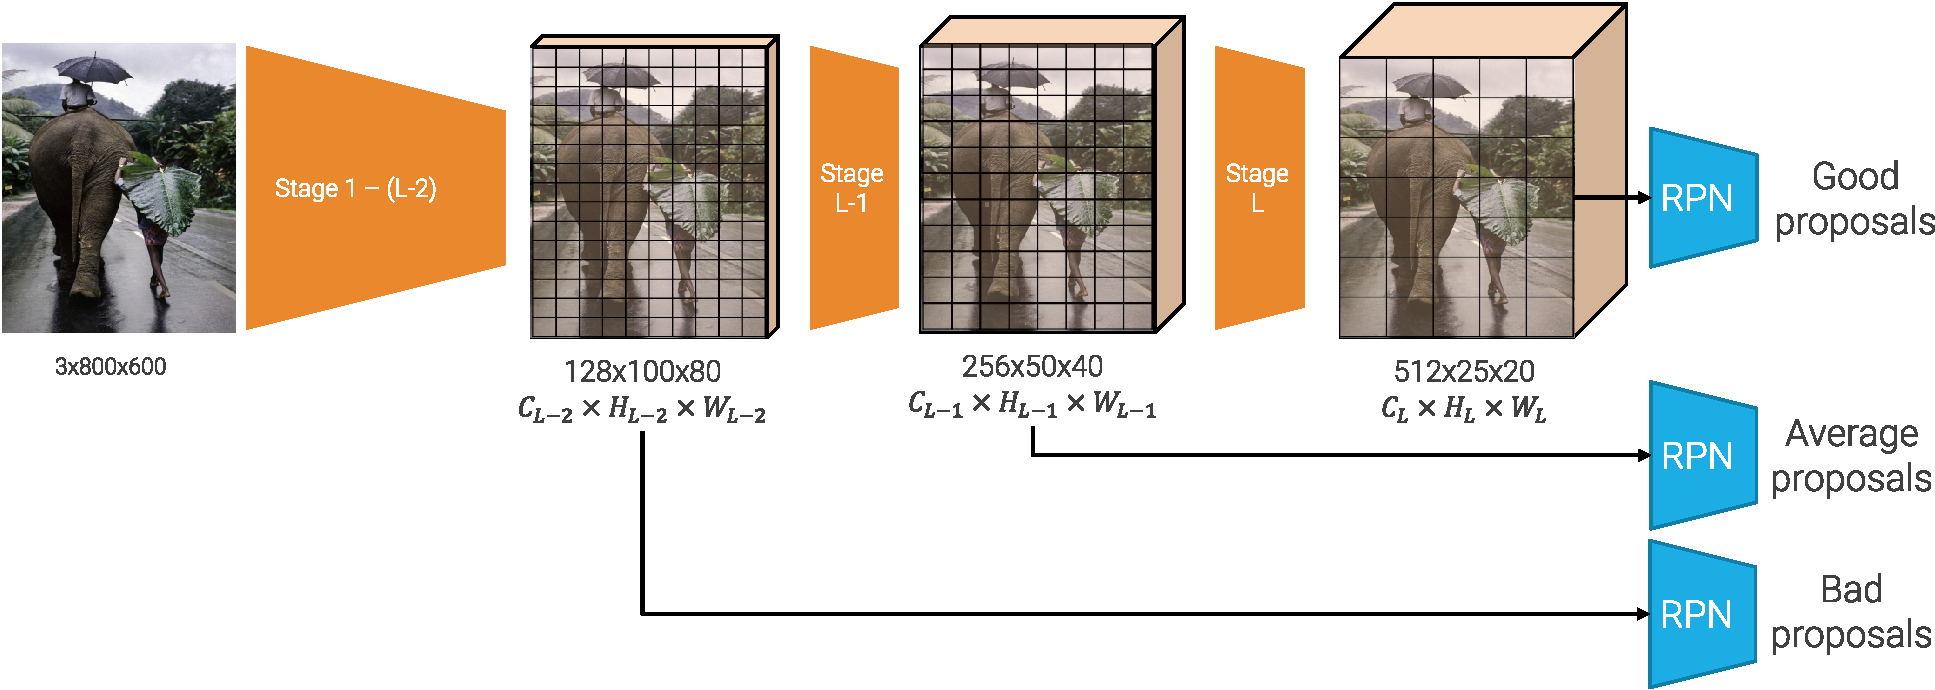
\includegraphics[width=0.8\linewidth]{./img/_cnn_pyramid_multi_scale.pdf}
        \end{figure}

    \item[Feature pyramid network (FPN)] \marginnote{Feature pyramid network (FPN)}
        Network that enhances small scale features (at the beginning of the network) by combining them with high resolution and semantically rich features (at the end of the network).

        \begin{figure}[H]
            \centering
            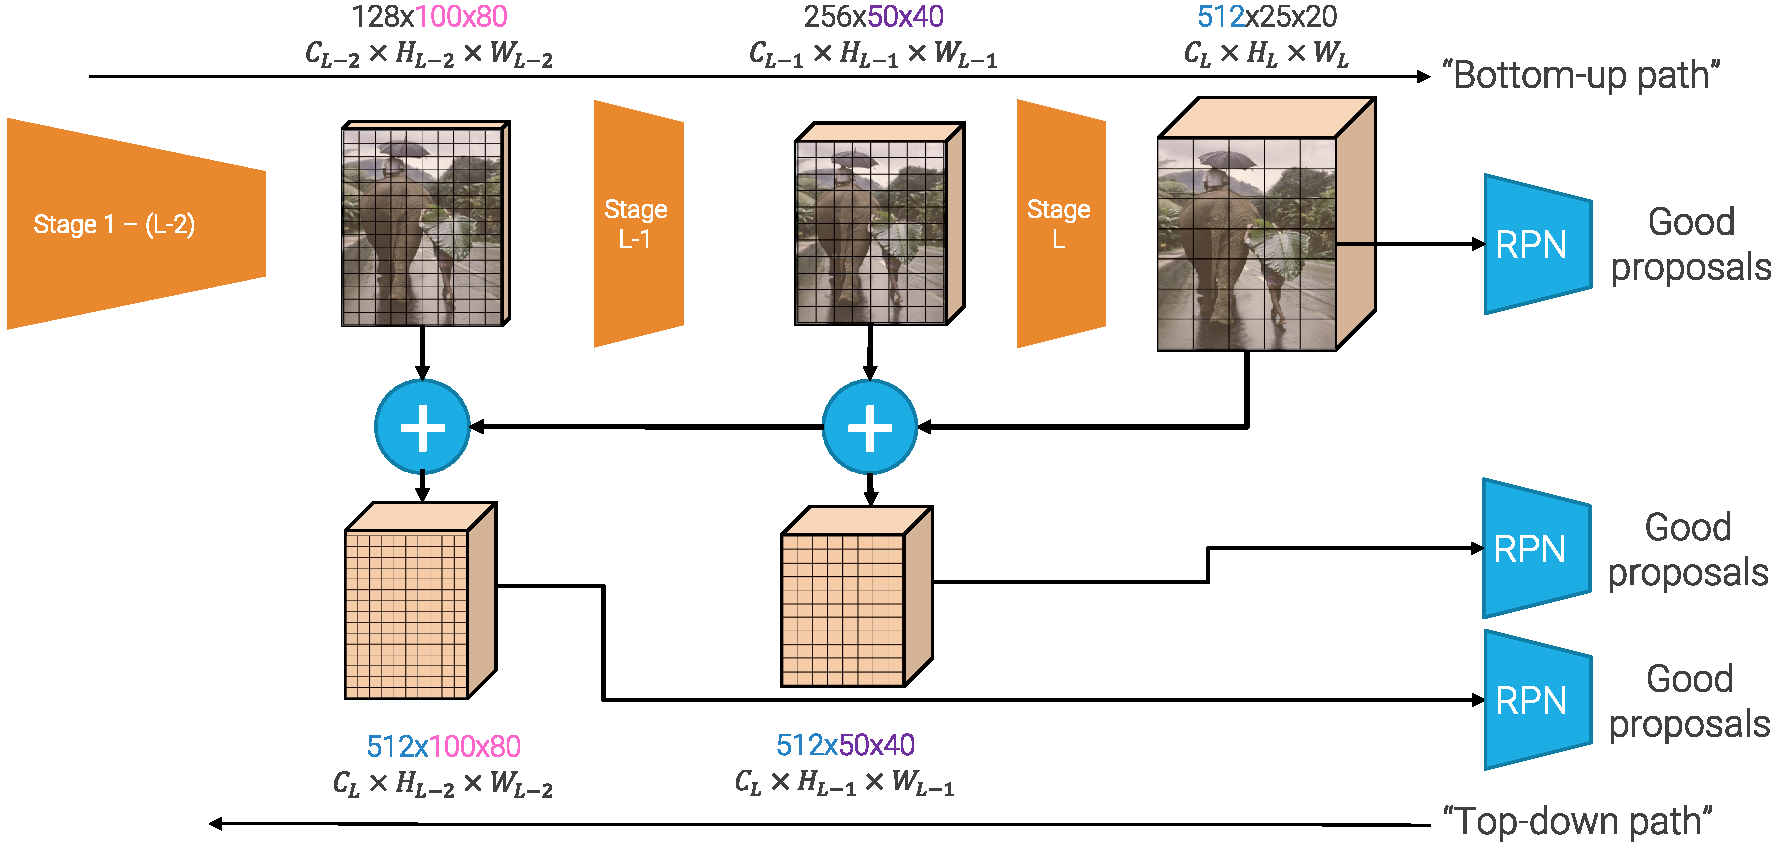
\includegraphics[width=0.7\linewidth]{./img/_fpn_flow.pdf}
            \caption{General FPN flow}
        \end{figure}

        \begin{description}
            \item[Top-down path] 
                Given the activation $A^{(L)}$ at layer $L$ and the activation $A^{(L-1)}$ at layer $L-1$, the top-down path computes the enhanced features as follows:
                \begin{enumerate}
                    \item Obtain $\bar{A}^{(L)}$ by upsampling $A^{(L)}$ using nearest neighbor to match the spatial dimension of $A^{(L-1)}$.
                    \item Obtain $\bar{A}^{(L-1)}$ by applying a $1 \times 1$ convolution to $A^{(L-1)}$ to match the number of channels of $A^{(L)}$.
                    \item Sum $\bar{A}^{(L)}$ and $\bar{A}^{(L-1)}$, and apply a $3 \times 3$ convolution to reduce aliasing artifacts caused by upsampling.
                \end{enumerate}

                \begin{figure}[H]
                    \centering
                    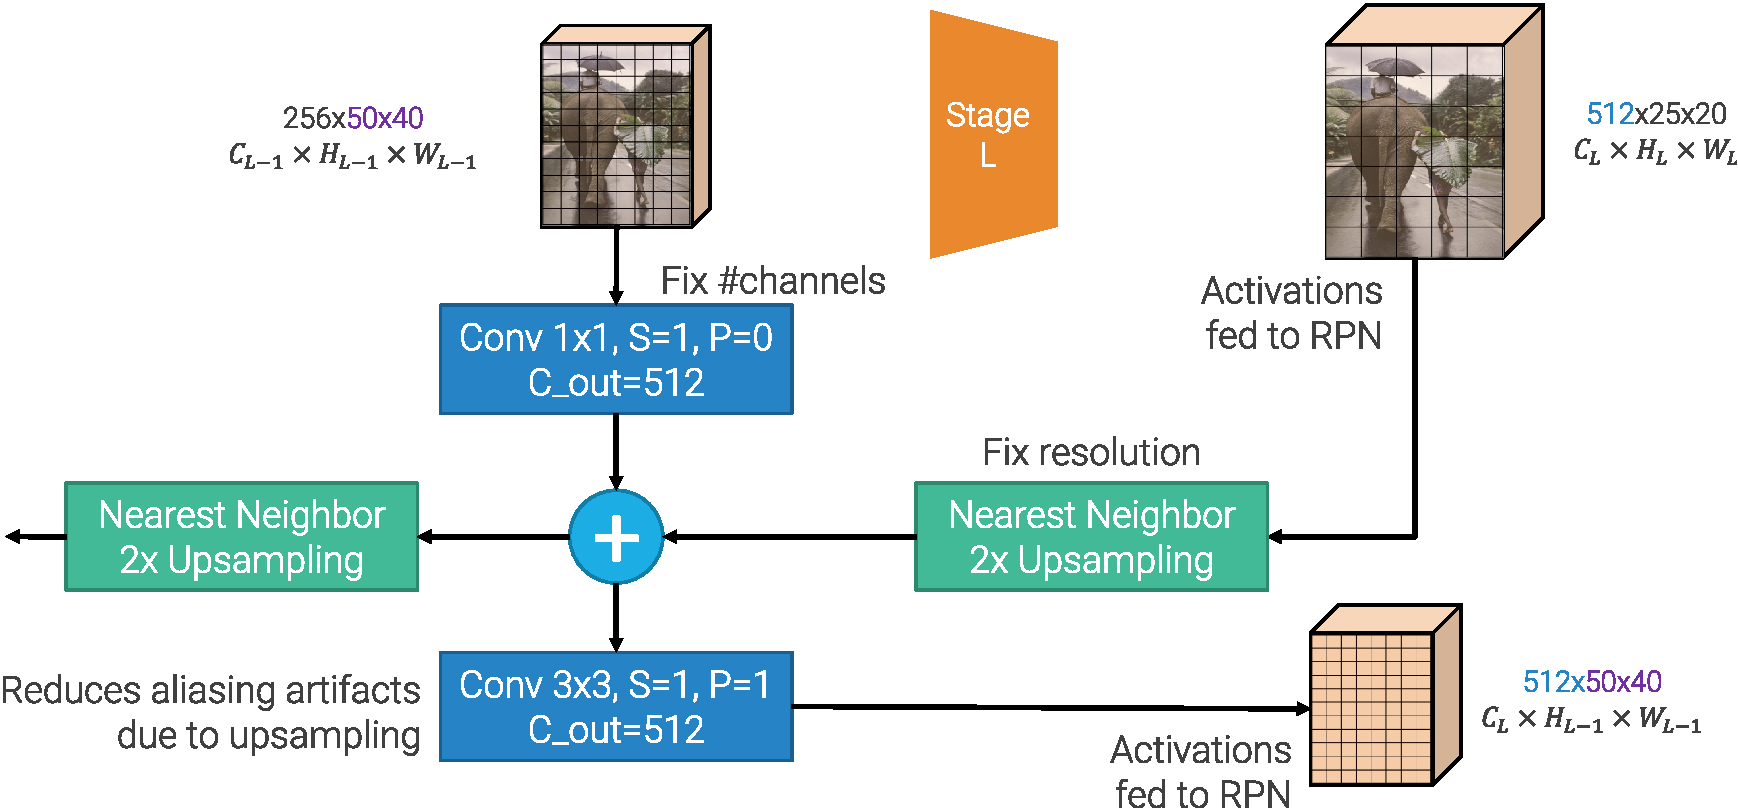
\includegraphics[width=0.65\linewidth]{./img/_fpn_top_down.pdf}
                    \caption{FPN top-down flow}
                \end{figure}
        \end{description}

    \item[Faster R-CNN with FPN] \marginnote{Faster R-CNN with FPN}
        The FPN is used with the feature extractor to obtain a pyramid of features $P_1, \dots, P_n$. A proposal of the RPN is assigned to the most suited level of the pyramid $P_k$.

        \begin{figure}[H]
            \centering
            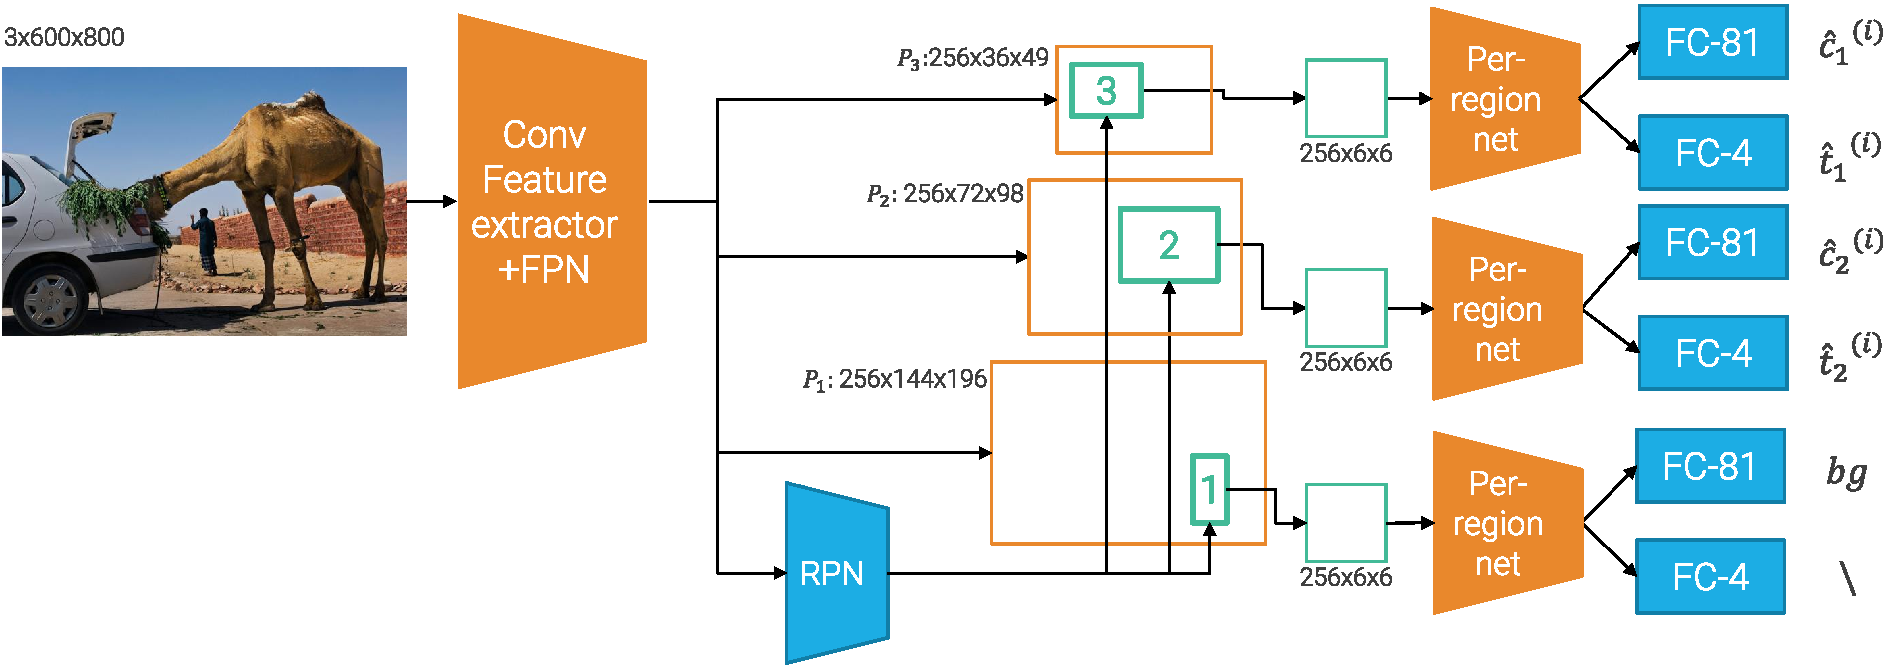
\includegraphics[width=0.8\linewidth]{./img/_faster_r_cnn_fpn.pdf}
            \caption{Example of faster R-CNN with FPN}
        \end{figure}

        \begin{remark}
            Given a proposal of the RPN with size $w \times h$, the most suited level of the pyramid $P_k$ is determined by the following formula:
            \[ k = \left\lfloor k_0 + \log_2\left(\frac{\sqrt{wh}}{224}\right) \right\rfloor \]
            where $k_0$ is the level of the feature map at which a $224 \times 224$ proposal should be mapped to.
        \end{remark}
\end{description}